%At the same time, research in the area of the Semantic Web has led to quite mature standards for modeling and codifying knowledge. Today, Semantic Web ontologies become a key technology for intelligent knowledge processing, providing a framework for sharing conceptual models about a domain. There are already powerful tools available for capturing and management of ontological knowledge~\cite{DuineveldEtal00}\cite{Knublauch04theprotege}. Moreover, the large and continuously growing amount of interlinked Semantic Web data has become a perfect match for novel data mining methods that employ link analysis due to their focus on relations between objects in addition to features/attributes of objects~\cite{KieferEtal2009}. Therefore, we propose to exploit the advances of the Semantic Web technologies to formally represent domain knowledge including structured collection of prior information, inference rules, knowledge enriched datasets etc, and thus develop frameworks for systematic incorporation of domain knowledge in an intelligent data mining environment. We call this technology the \emph{semantic data mining}.
Annotation in general (traditionally) is a summary made of information in some source such as document, online record, image, video and so forth. With the emergence and development of the Semantic Web, there have been increasing demands for \emph{semantic annotation}, a kind of meta-data derived based upon specific knowledge about the world, rather than indifferent to any ontological commitments. In other words, semantic annotation aims at assigning to the basic element of information links to formal semantic descriptions~\cite{KiryakovEtal04}. Such elements should constitute the semantics of their source, for example, named entities in a document, certain part of an image depicting someone's head portrait.

Semantic annotation is crucial in realizing semantic data mining by bridging formal semantics in Semantic Web meta-data with data. The majority of data underpinning a wide spectrum of data mining applications are stored in various formats, including structured sources such as relational databases (RDB) with their proven track record of scalability and reliability, or semi-structured sources such as spreadsheets with their advantage of low maintenance and cheaper overheads, or even unstructured sources such as text corpus. The problem of how to impart knowledge encoded in Semantic Web ontologies to all sorts of data becomes a major challenge in realizing the semantic data mining. We believe \emph{semantic annotation} is the solution to this challenge. It aims at assigning semantic descriptions to elements of data. To ease the burden of common users that are not familiar with the Semantic Web, we develop a learning-based semantic search algorithm to suggest appropriate semantic descriptions for annotation.

%thesis-semantic-annotation-workflow
\begin{figure}[tbh]
\begin{center}
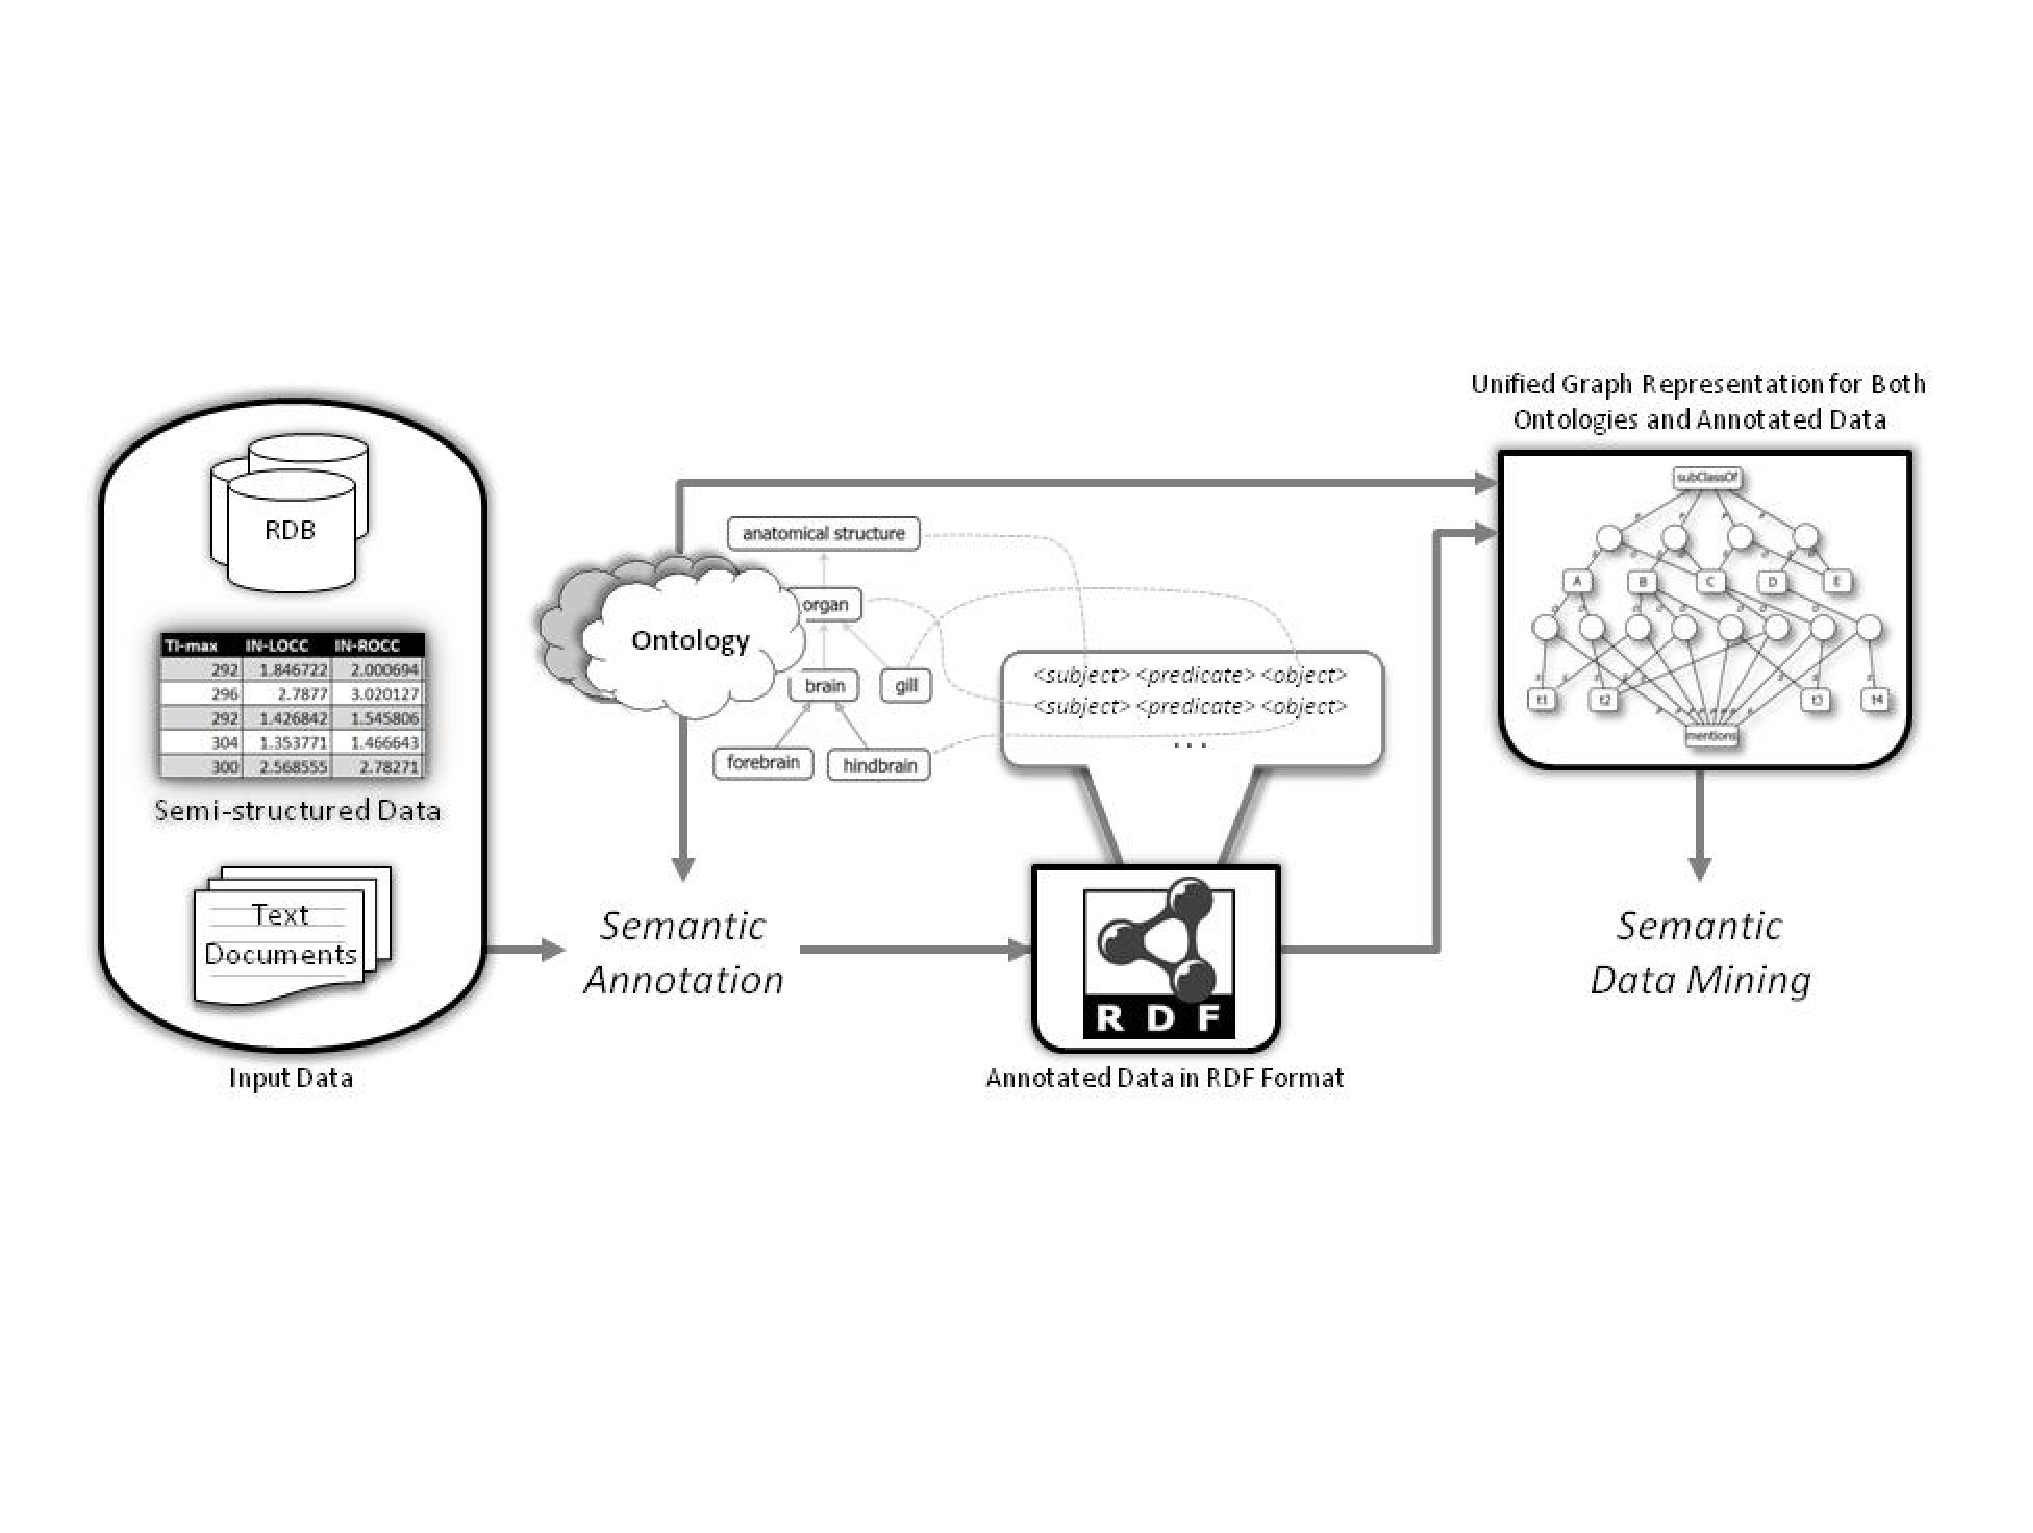
\includegraphics[width=\textwidth, trim=0 7cm 0 6cm, clip=true]{fig/thesis-semantic-annotation-workflow.eps}
\end{center}
\caption[Semantic annotation in the workflow of semantic data mining.]{\label{fig:annotation-workflow} Data stored in different sources (e.g., relational databases, spreadsheets, texts etc) are semantically annotated. The output is in RDF format where elements of data are linked to formal semantic descriptions in ontologies. Annotated data and ontologies together are then represented in a unified graph representation for subsequent analysis in semantic data mining.}
\end{figure}

\section{Automatic Annotation by Semantic Search}
Semantic annotation is crucial in realizing semantic data mining by bringing meanings to data. The function of semantic annotation in the workflow of a semantic data mining system is illustrated in Figure~\ref{fig:annotation-workflow} Annotating unstructured data (e.g., text) has been studied more extensively than annotating (semi-)structured data due to the proliferation of information extraction techniques that facilitate automatic entity recognition from text. Since large amount of data for knowledge discovery applications are stored in (semi-)structured sources, we focus on annotating (semi-)structured data.

The annotation process can be generally divided into two steps. The first is to establish mappings between existing Semantic Web terms and terms need to be annotated in the data. The second step is to come up with a local ontological structure constituting the semantic web terms to model the data.

Most of previous work in annotating (semi-)structured data focus on the second step. Some skip the first step and bootstrap the ontological terms and structure from the local data itself. For example, a number of systems that map data in RDB to RDF format leverage a set of rules such as ``table to class and column to predicate". Bernes-Lee expands the rule as follows~\cite{TBL98}: 1) An RDB record is a RDF node. 2) The column name of an RDB table is an RDF predicate. And 3) An RDB table cell is a value. Other examples of rules involved in mapping RDB schema to OWL ontology include ``foreign keys to object property and non-key attributes to datatype property".
Similar idea has been adopted in annotating spreadsheets as well. Existing spreadsheet-to-rdf tools typically map spreadsheets to star-shaped RDF graphs, i.e., each row is an instance, with each column representing a property. Some tools try to express richer spreadsheet semantics, e.g., Han et al. developed a spreadsheet-to-rdf tool called RDF123~\cite{RDF123} that allows users to define mappings to arbitrary graphs.

We argue that mapping RDB or spreadsheet to linked data (e.g., RDF) without referencing to existing semantic descriptions does not lend itself well to aiding semantic data mining. The automatically constructed self-contained local ontology may be applicable to describe a specific dataset but is most likely too rough to capture the full domain semantics that is necessary to express meaningful domain knowledge. Moreover, with the advent of the Semantic Web and pervasive connectivity, an increasing number of ontologies has been made widely available for reuse. These ontologies are created by thorough knowledge engineering process and should serve as better models for annotation. However, on the other hand, the sheer number of Semantic Web ontologies and lack of effective search functionality can lead to a huge hidden barrier for common users. Choosing proper Semantic Web ontologies and terms (classes and properties) requires familiarity with appropriate ontologies and the terms they define. There is very few system that is able to provide automatic suggestions. To solve this problem, we propose a learning-based semantic search algorithm to suggest proper Semantic Web terms and ontologies for annotation given semantically related words and general domain and context information.


%
%The TopBraid Composer [6] Semantic Web development system can extract
%class and instances information from spreadsheets and these can be further manipulated
%and transformed using additional tools in the suite.
%One limitation of the approaches described above is that the RDF schema
%used for one row or a group of rows is quite simple, usually having the shape of a
%star in which all property edges come out from a single center �C the ID resource.
%This works well for normalized database tables, but is not flexible enough for
%general purpose spreadsheets. Another limitation in the above approaches is that
%one fixed RDF schema is applied to all rows of a table.



\subsection{Proposed Learning-based Semantic Search Algorithm}
In order to suggest suitable Semantic Web terms and ontologies for users to annotate their data, we propose a learning-based semantic search algorithm. We first submit a list of terms appeared in the schema of (semi-)structured data to our semantic search algorithm and then use the returned results for annotation. In a fully automatic setting, the search algorithm is configured to return the top-1 hit; while in an interactive setting, the search algorithm returns ordered top-k search results for users to decide. Previous semantic search algorithms leverage a variety of measures, including lexical and structural similarities (see details below) to rank Semantic Web documents according to how likely they can be semantically matched to the search terms. However, using any single measure alone may not be sufficient to achieve the optimal result. We propose to combine various measures to a weighted feature-based search model, where the weights are learned from training data. We believe the incorporation of learning techniques will improve the semantic search result.

\subsubsection{Feature-based Semantic Search Model.}
\label{FeatureModel}
Consider a set of ontologies $\mathbf{O}=\{O_1...O_m\}$ returned as the search result for a specific search term. Let
$\mathbf{\Phi} = \{\phi_1(O_i)...\phi_m(O_m)\}$ be a vector of real-valued feature functions $\phi~:~O\mapsto \mathbb{R}$
that compute rank indicating how ontologies should be ordered in the search result. The one with the highest rank is the top-hit for a specific search. Let $\mathbf{W} =\{w_1...w_m\}$
be a vector of real-valued weights associated with each feature.
A score is computed for each ontology $O_i$ by
taking the dot product of the features and weights:
$$\tau(O_i,\mathbf{W})=\mathbf{\Phi} \cdot \mathbf{W} \; .$$
We can leverage a variety of ranking methods proposed in the literature as the feature functions $\mathbf{\Phi}$. For example,
Alan et al.~\cite{AlaniEtal05} proposed four types of measurements to evaluate the ranks for ontologies given a list of search terms: The Class Match Measure (CMM) measures the coverage of an ontology of the given search terms; The Centrality Measure (CEM) is aimed to asses how representative a class is of an ontology according to the assumption that the more central a class is in the hierarchy, the more likely it is well analyzed and represented; Density Measure (DEM) examines how well a concept is represented by taking into consideration its neighboring concepts; And Semantic Similarity Measure (SSM) calculates the distance between classes  in an ontology that match the search terms.
The Swoogle search engine~\cite{Ding05searchon}\cite{Ding05findingand} weighs different types of links between Semantic Web data and rank them using link-based algorithms to evaluate the importance of Semantic Web objects at three levels of granularity: documents terms and RDF graphs.
Maedche et al.~\cite{Maedche03Onto} described a two level similarity measure. The first level is the so called lexical comparison level, where a lexical similarity measure, called string matching (SM), is proposed based on Levenshtein's edit distance to compare two lexical entries $L_i$ and $L_j$:
$SM(L_i,L_j)=max\left( 0, \frac{min\left(|L_i|,|L_j| \right)-ed\left(L_i,L_j\right)}{min\left(|L_i|,|L_j|\right)} \right)$
$\in \left[0,1\right]$. The second level is the conceptual comparison level where two taxonomies are compared by examining the semantic cotopies of the sets of concepts from the two ontologies.

\subsubsection{Training Set.}
Our algorithm to determine the vector of weights $\mathbf{W}$ requires a \emph{training set} of known
top hit in the search result (chosen by human):
$$\mathcal{T}=\{<\mathbf{O}^1,l_1>...<\mathbf{O}^n,l_n>\} \; ,$$
where each set of ontology namespaces $\mathbf{O}^i=\{O_1...O_k\}$ is associated with label $l_i \in \{1...k\}$,
indicating which of the ontologies should be selected for annotating the specific term $t_i$ (i.e.,
$O_{l_i} \in O$ is the true ontology selected by human as the best choice for annotating the term).
There are several ways to estimate $\mathbf{W}$ from the training set $\mathcal{T}$ as described below.


\subsubsection{Subgradient Descent.}
We can view the weight learning as maximum margin structured learning problem. Given a training set and loss function,
the learned $\mathbf{W}$ should score each known top-hit result $O_{l_i}$ higher than all other $O$ by at least
$\mathcal{L}(O_{l_i}, O)$, where $\mathcal{L}$ is the loss function. Mathematically, this constraint is
$$\forall i, O \in \{\mathbf{O}^i\backslash O_{l_i}\}, \mathbf{W}\cdot \mathbf{\Phi}(O_{l_i}) \geq \mathbf{W}\cdot \mathbf{\Phi}(O)+\mathcal{L}(O_{l_i}, O) \; ,$$
where $\{\mathbf{O}^i\backslash O_{l_i}\}$ is the set of possible ontologies returned by a specific search query excluding the gold standard ontology $O_{l_i}$ chosen by human. We can express this constraint as the following convex program:
$$\min_{\mathbf{W},\zeta^i}\frac{\lambda}{2}\|\mathbf{W}\|^2+\frac{1}{d}\sum^d_{i=1}\zeta^i$$\\
$$s.t. \forall i, O \in \mathbf{O}, \mathbf{W} \cdot \mathbf{\Phi}(O_{l_i})+\zeta_i \geq \mathbf{W} \cdot \mathbf{\Phi}(O) + \mathcal{L}(O_{l_i},O) \; ,$$
where $\lambda$ is a regularization term that prevents overfitting. We can rearrange the convex program to show that the optimal $\mathbf{W}$ minimizes
\begin{equation}
c(\mathbf{W})=\frac{1}{d}\sum^d_{i=1}r^i(\mathbf{W})+\frac{\lambda}{2}\|\mathbf{W}\|^2 \; ,
\label{convex}
\end{equation}
where $r_i(\mathbf{w})=\max_{O\in \{O_{l_i}\}}(\mathbf{W} \cdot \mathbf{\Phi}(O) + \mathcal{L}(O_{l_i},O)) - \mathbf{W} \cdot \mathbf{\Phi}(O_{l_i})\; .$
This objective function is convex but nondifferentiable. We can therefore minimize it with subgradient descent, an extension of gradient descent to nondifferentiable objective functions. The subgradient of Equation~\ref{convex} is
$$\lambda \mathbf{W} + \frac{1}{d}\sum^d_{i=1}(\mathbf{\Phi}(O^\ast_{l_i})-\mathbf{\Phi}(O_{l_i})) \; ,$$
where $O^\ast_{l_i}=argmax_{O \in \{ O_{l_i} \} } \mathbf{W} \cdot \mathbf{\Phi}(O) + \mathcal{L}(O_{l_i}, O)$ is the predicted top hit ontology.
%, determined by the loss function $\mathcal{L}(O_{l_i}, O)$ and current $\mathbf{W}$.
Based on these ideas, we can iteratively compute the subgradient of equation~\ref{convex}~\cite{Ratliff07subgradient} and converge at the optimal weights.


\subsubsection{Logistic Regression.}
The second method is based on logistic regression (sometimes
called maximum entropy classification). We
modify the traditional logistic regression loss function to
rank, rather than classify, instances.
Let the binary random variable $C_i$ be 1 if and only if
ontology $O_i$ is the gold standard chosen by human.
Given $\mathbf{W}$ and $\mathbf{\Phi}$, we can compute the
probability of $C_i$ as follows:

$$p\left(C_i=1|\mathbf{O, W}\right)=\frac{e^{\tau(O_i, \mathbf{W})}}{\sum_{O_j \in \mathbf{O}} e^{\tau(O_j, \mathbf{W})}} \; ,$$
where the score for ontology $O_i$ is normalized by the scores for
every other ontologies.
We can estimate $\mathbf{W}$ from the training set $\mathcal{T}$
by minimizing the negative log-likelihood of the data given $\mathbf{W}$:
\begin{equation}
\mathcal{L}\left(\mathbf{W}, \mathcal{T}\right) = - \sum_{O^i \in \mathcal{T}} \log p \left(C_{l_i}|\mathbf{O,W} \right) \; .
\label{logisticregression}
\end{equation}
Note that this is the sum of probabilities for each of the gold standard ontology
 for the current setting of $\mathbf{W}$. We can also
add a Gaussian prior over $\mathbf{W}$ with fixed mean and variance
to mitigate over-fitting. We can find the setting of $\mathbf{W}$ that minimizes
Equation~\ref{logisticregression} using limited-memory BFGS, a gradient
ascent method with a second-order approximation~\cite{Liu89onthe}.

\section{Annotation by Multiple Ontologies}
%%general review of the field of ontology matching
The presence of heterogeneity among schemas supporting vast amount of information demands advanced solution for semantic integration of disparate data sources to facilitate interoperability and reuse of the information. The challenge is especially pronounced in many scientific domains where a massive amount of data are produced independently and thus each having their own data vocabulary. While manual integration is time-consuming and requires expensive specialized human capital, the development of automatic approaches becomes imminent to aid inter-institute collaborations. One purpose of the present paper is to suggest a method for solving a specific kind of ontology matching problem under some severe constraints that can cause traditional methods to be ineffective. The constraints that we deal with are, namely, 1) little-to-no string-based or linguistic similarity between terminologies, and 2) all numeric typed data instances. This phenomenon is commonly seen in integrating scientific datasets which involves discovery of correspondences among distinct numeric-typed summary features (``attributes") that are used to characterize datasets that have been collected and analyzed in different research labs. We call this the \emph{attribute matching} problem.

Our study of matching alternative attribute sets is closely related to the schema matching problem. According to the type of instance value, various instance-based approaches have been developed in previous research. For example, for textual attributes, a linguistic characterization based on information retrieval techniques can be applied~\cite{Rahm01asurvey}; for nominal attributes, evaluation of the degree of overlap of instance values is a preferred approach. Larson et al.~\cite{Larson1989} and Sheth et al.~\cite{Sheth1988} discussed how relationships and entity sets could be integrated primarily based on their domain relationships. Similarity of partially overlapped instance set can be also calculated based on measures such as Hamming distance and Jaccard coefficient; for numeric attributes, most methods use aggregated statistics to characterize the attributes, e.g., `SSN' and `PhonNo' can be distinguished based on their respective patterns~\cite{Rahm01asurvey}. Hybrid systems that combine several approaches to determine matching often achieve better performance. For example, SemInt~\cite{Li00semint:a} is a comprehensive matching prototype exploiting up to 15 constraint-based and 5 content-based matching criteria. The LSD (Learning Source Descriptions)~\cite{Doan2000} system uses several instance-level matchers (learners) that are trained during a preprocessing step. The iMAP~\cite{Dhamankar04imap} system uses multiple basic matchers, called searches, e.g., text, numeric, category, unit conversion, each of which addresses a particular subset of the match space.

Due to the nature of many scientific datasets, we face several unique challenges. First, the data under study are semi-structured, thus invalidating those matching methods that presume a complete, known-in-advance schematic structure. In addition, totally different labels (usually acronyms or pseudowords) are widely adopted for the same or similar metrics, rendering lexical similarity-based methods unsuitable. Moreover, an important limitation of previous instance-based matching methods is their inability to handle numerical instances appropriately in certain domain applications. They use statistical characterization extracted from the numerical instances, such as range, mean and standard deviation, to determine match. However such information is too rough to capture patterns in data that are crucial in determining the correspondence.

To solve this difficulty, in the present paper, viewing the two matching problems as combinatorial optimization problems with distinct yet interrelated objective functions, we propose a novel approach using a multi-objective heuristics to discover attribute matching and cluster matching simultaneously. The objectives in the optimization are to minimize distances of attribute matching and cluster matching respectively. We explore the widely used simulated annealing algorithm as the metaheuristics algorithm and briefly compare its performance with the evolutionary multi-objective algorithm in experiments.

\emph{Density Profile}: To represent clusters using density profiles, the attribute's range in each cluster is first discretized into a number of bins, and the similarity between two clusters corresponds to the number of points of each cluster falling within these bins. The formal definition for this number of points is the \textit{density} of an attribute-bin region for cluster $c_k$ in clustering $C$, denoted as $dens_C(k, i, j)$. It refers to the number of points in the region $(i, j)$---the $j$-th bin of the $i$-th attribute---that belongs to the cluster $c_k$ of clustering $C$. For example, for clustering $C$ in Fig.~\ref{fig:density_profile}, $dens_C(1, 1, 1) = 8$, because there are 8 data points in region $(1, 1)$---the first bin of the first attribute $x$---that belongs to the first cluster $c_1$.

%The values of $dens_C(k, i, j)$ for all possible $k$, $i$, $j$ are then listed in a certain ordering to form a clustering's \emph{density profile vector} (defined below). This ordering is imposed on all attribute-bin regions and must be applied to the two datasets in which the clusterings were generated. It is necessary, then, that both datasets must have the same attribute set. If this requirement does not stand, the matching between the sets must be specified in advance. Therefore, in order to apply the density profile method in the ERP pattern matching problem, we must first carry out measure matching. We further discuss the interdependence between pattern matching and metric matching in Section~\ref{sec:discuss}.

The density profile vector $V_C$ for a clustering $C$ is formally defined as an ordered tuple:
\begin{align}
\notag V_C = \bigg[ & dens_C(1, 1, 1), ~\ldots, ~dens_C (1, 1, Q),\\
\notag & dens_C (1, 2, 1), ~\ldots, ~dens_C (1, M, Q),\\
& dens_C (2, 1, 1), ~\ldots, ~dens_C (N, M, Q) \bigg]\, ,\label{eq:densp}
\end{align}
where $Q$ is the number of bins in each of the $M$ attributes, and $N$ is the number of clusters in $C$.

\emph{The ADCO measure}: After the density profile vectors of two clusterings $C$ and $C'$ are obtained, the degree of similarity between  $C$ and $C'$ can be determined by calculating the dot product of the density profile vectors:
$sim(C, C') = V_C  \cdot V_{C'} \, .$

The $ADCO(C,C')$ measure is defined as $sim(C,C')$ normalized by the maximum achievable similarity when using either of the two clusterings:
\[ADCO(C, C') = \frac{sim(C, C')}{NF(C, C')} \, , \]
where $NF(C, C') = max \big[sim(C, C), \,sim(C', C')\big]$.

\begin{figure}[tb]
\begin{center}
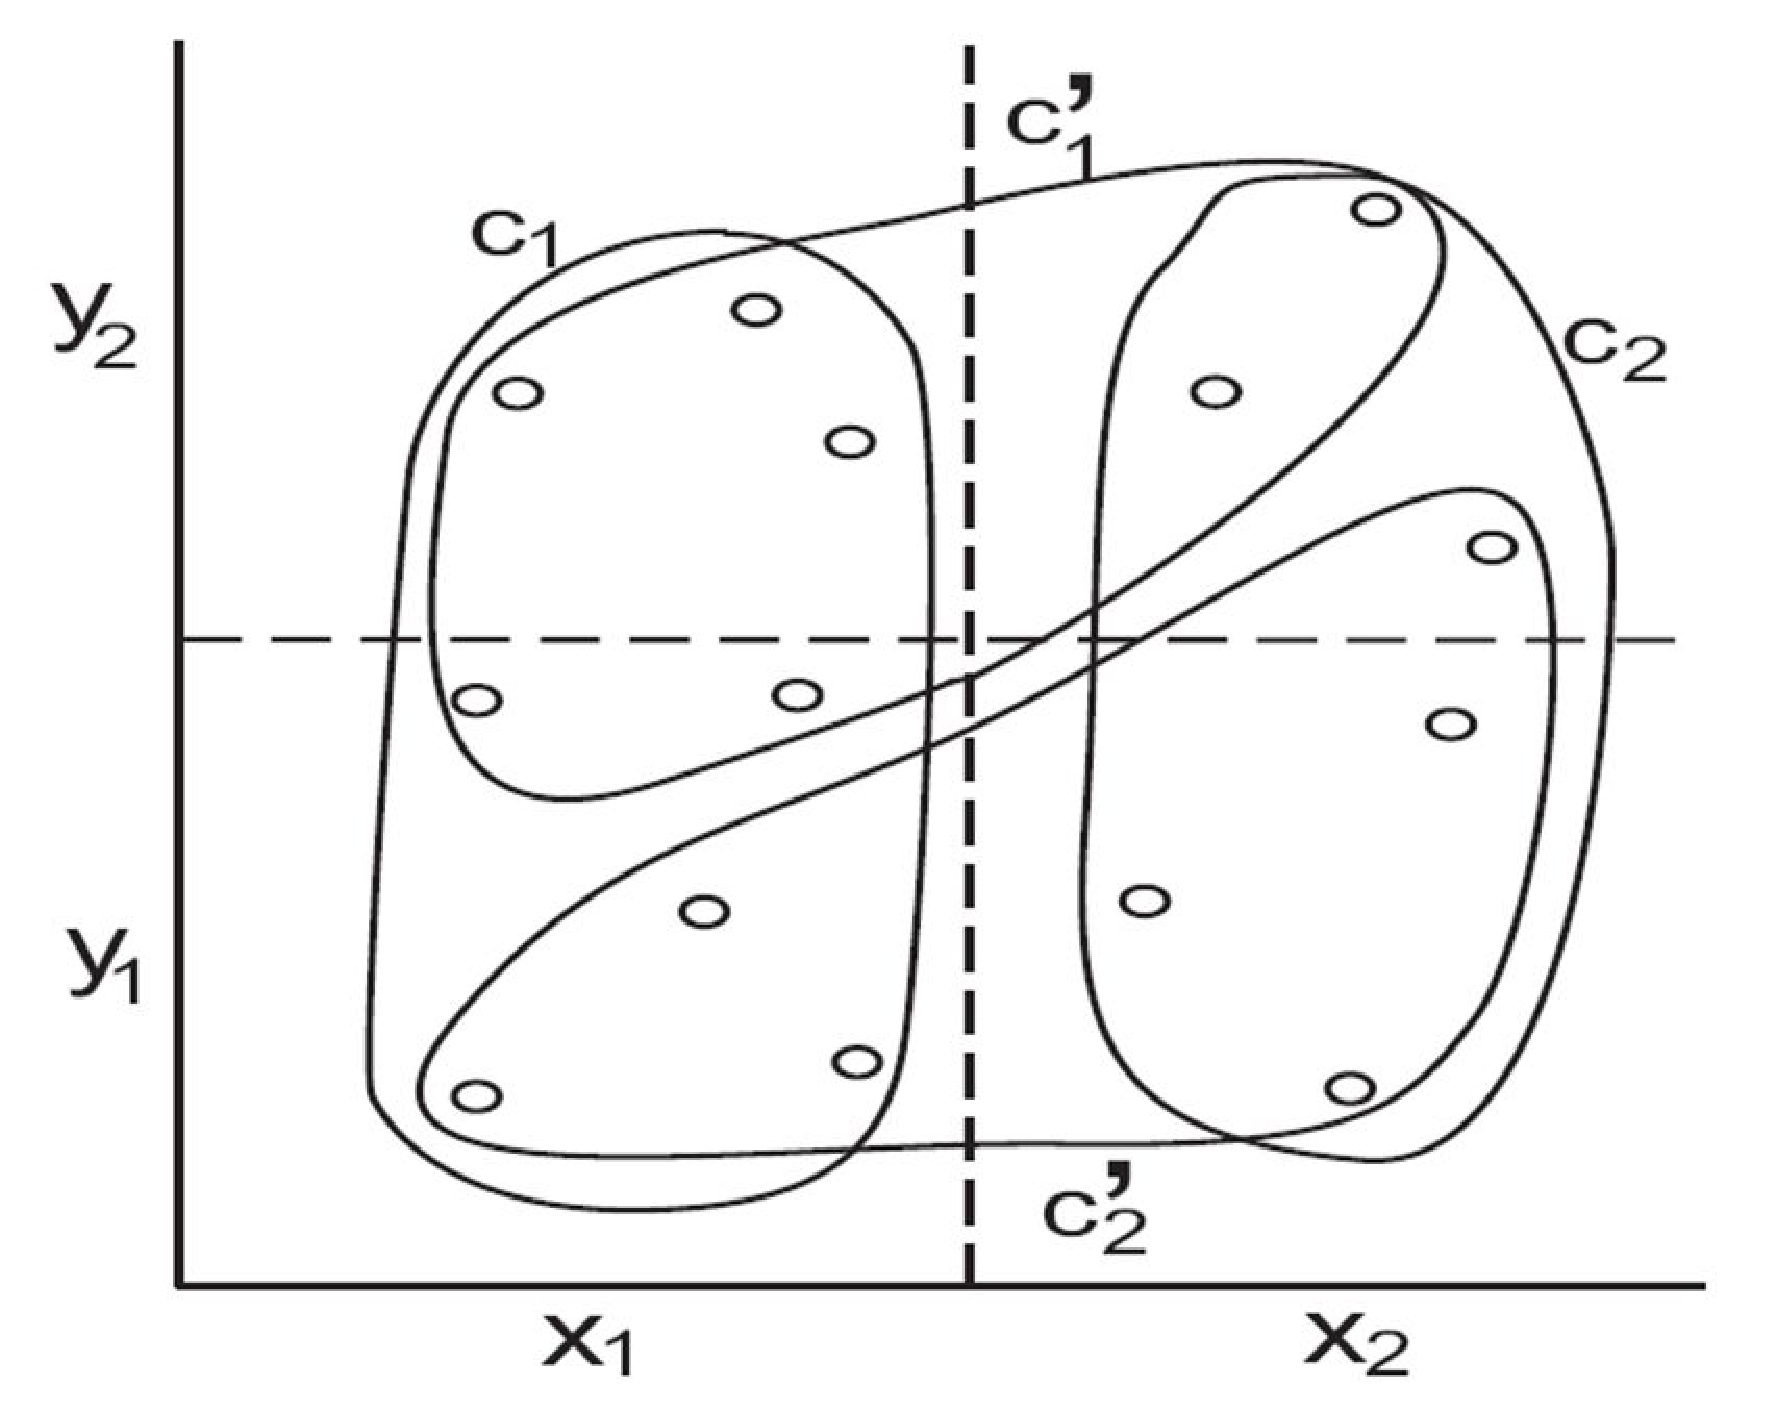
\includegraphics[width=0.4\textwidth]{fig/density_profile.eps}
\end{center}
\caption[An example of cluster density profiles]{\label{fig:density_profile} Two clusterings $C=\{c_1, c_2\}$ and $C'=\{c_1', c_2'\}$. Two attributes $X$ (attribute 1) and $Y$ (attribute 2) are discretized into 2 bins each. See~\cite{Bae2010} for details.}
\end{figure}

\subsection{The Multi-Objective Simulated Annealing Framework}
\textbf{Problem Definition:} We tackle two integration tasks in this work, namely, the attribute matching and cluster matching problems. We cast the dual matching problems to a multi-objective optimization problem so that the matchings can be solved simultaneously. The two objective functions to be optimized are defined as the total distance of matched elements in attribute and cluster matching respectively. To this end, we explore methods to represent attributes and clusters so that distance measure can be reasonably defined. We assume that the optimal matching lies at the Pareto front in this multi-objective problem.

We use metaheuristics search algorithm to solve this multi-objective optimization problem. In the following we describe the widely used simulated annealing algorithm and how it can be adapted to multi-objective optimization and applied to solve the matching problems. Later in the Experiment Section, we briefly describe an evolutionary multi-objective algorithm and compare their performance.

To solve the dual matching problems, we adopt a strategy of multi-objective simulated annealing (MOSA) described in~\cite{Suman2003}, in which the acceptance criterion in the simulated annealing process is established based on the idea of Pareto-domination based fitness. Fitness of a solution is defined as one plus the number of dominating solutions in Pareto-optimal set. The larger the value of fitness, the worse is the solution. Initially, fitness difference between the current and the generated solution is less and the temperature is high so any move is accepted due to both of them. This gives a way to explore the full solution space. As the number of iterations increases, temperature decreases and fitness difference between the current and generated solutions may increase. Both of them make the acceptance move more selective and it results in a well-diversified solution in true Pareto-optimal solutions. Details of our adaptation of the above multi-objective simulated annealing framework is outlined in Algorithm~\ref{MOSA}.


%\subsection{Simulated Annealing}
\begin{algorithm}
\caption{Multi-Objective Simulated Annealing}
\label{MOSA}
\begin{algorithmic}
\REQUIRE Empty Pareto-optimal set of solutions $\mathbf{\Sigma}$
\REQUIRE Empty current decision vector $\mathbf{X}=[x_a,x_c]$
\REQUIRE Initial temperature $T$
\STATE $count=0$
\WHILE{$T > threshold$}
\STATE $initialize(\mathbf{X})$ \hspace{1in} %$//\mathbf{X}^0=[x_a^0,x_c^0]$
\STATE Put $\mathbf{X}$ in $\mathbf{\Sigma}$
\STATE $\mathbf{X}'=generate\_solution(\mathbf{X})$
\STATE $S_{\mathbf{X}'}=evaluate\_solution(\mathbf{X}')$
\STATE $\Delta S = S_{\mathbf{X}'} - S_X$
\IF{$r=rand(0,1)<exp(\frac{-\Delta S}{T})$}
\STATE $\mathbf{X}=\mathbf{X}'$
\STATE $S_X=S_{X'}$
\ENDIF\\
\STATE count = count + 1
\STATE //Periodically restart
\IF{$count == restart\_limit$}
\STATE $\mathbf{X}=select\_random\_from\_Pareto(\mathbf{\Sigma})$
\STATE continue
\ENDIF
\STATE $reduce\_temperature(T)$
\ENDWHILE
\end{algorithmic}
\end{algorithm}

Mathematically, the processes involved in the proposed multi-objective simulated annealing framework can be defined as follows.
\begin{align}
\notag X&=[x_a, x_c]\\
\notag F&=[f_a, f_c]\\
\notag P_a([x_a^{(n-1)},x_c^{(n-1)}])&=[x_a^{(n)}, x_c^{(n-1)}]\\
\notag P_c([x_a^{(n-1)},x_c^{(n-1)}])&=[x_a^{(n-1)}, x_c^{(n)}]\\
\notag G_{c|a}([x_a^{(n)},x_c^{(n-1)}])&=[x_a^{(n)}, x_c^{(n)}]\\
\notag G_{a|c}([x_a^{(n-1)},x_c^{(n)}])&=[x_a^{(n)}, x_c^{(n)}]\\
\notag G\circ P([x_a^{(n-1)},x_c^{(n-1)}])&=[x_a^{(n)}, x_c^{(n)}]
%F(X^{(n)})&=[f_a(x_a^{(n)}), f_c(x_c^{(n)})]
\end{align}
$X$ is the decision vector that contains two variables for attribute matching, $x_a$, and cluster matching, $x_c$, respectively (details in Section~\ref{sec:variables}). $F$ is the objective function vector that contains two criterion functions ($f_a$ and $f_c$) to evaluate attribute matching and cluster matching decisions (details in Section~\ref{sec:obj_funcs}). $P$ is the random perturbation function that takes a decision vector in the $(n-1)$th iteration and partially advances it to the $n$th iteration (we use $P_a$ or $P_c$ to distinguish between the random selections). The partial candidate decision generation function $G$ takes the output of $P$ and fully generate a decision vector for the $n$th iteration (by advancing the left-out variable in $P$ to its $n$th iteration). Thus, the compound function $G\circ P$ fulfils the task of generating an $n$th-iteration candidate decision vector given the $(n-1)$th one (details in Section~\ref{sec:new_sols}).
\subsection{Decision Variable}
\label{sec:variables}
The domains of the decision variables in the matching problems take values on a permutation space. In other word, by formalizing the problem of finding correspondent elements of two sets $S$ and $S'$ of cardinality $n$ as an optimization problem, the solution is completely specified by determining an optimal permutation of ${1,\ldots,n}$. For instance, for two sets of three elements, their indexes range over $\{0, 1, 2\}$. Applying a permutation $\pi =\{2, 0, 1\} \in S_3$ on $S'$ can be viewed as creating a mapping (bijection) from elements on the new positions of $S'$ to elements on the corresponding positions in $S$. %This mapping underlies the correspondence we try to discover in the matching problem.
In this example, the permutation $\pi$ on $S'$ specifies the following correspondences: $S_0 \leftrightarrow S'_2$, $S_1 \leftrightarrow S'_0$, and $S_2 \leftrightarrow S'_1$.

Formally, let $P_n$ ($n\in \mathbb{N}$) be the symmetric group of all permutations of the set $\{1, 2, \ldots, n\}$. Given two sets $S$ and $S'$ with the same cardinality of $n$, performing identity permutation on one set and an arbitrary permutation $\pi \in S_n$ on the other specifies a matching (or mathematically speaking, mapping) between the two sets.
In the multi-objective optimization formalism for solving attribute matching and cluster matching problems, the decision vector has two variables: $X=[x_a, x_c]$. If we have $M$ attributes and $N$ clusters to match respectively, then $x_a \in P_M$ and $x_c\in P_N$.

%Let us first define $\rho$ as the stochastic permutation of a subscript index set. Without causing confusion, we also define function $\rho(k)$ that returns the value at index $k$ in the permutation set. (i.e., $\rho = \{\rho(1), \rho(2), ... \rho(n)\}$ is the permutation of $\{0, 1, ..., n\}$.) We can view $\rho$ as a correspondence function between set $S_k$ and $S'_{\rho(k)}$, assuming correspondent positions in each set are considered to map to each other. For instance, if two sets both have three elements, then the subscript index set ranges over $\{0, 1, 2\}$. Supposing $\rho$ returns $\{2, 0, 1\}$, we can then obtain following matchings: $S_0 \leftrightarrow S'_2$, $S_1 \leftrightarrow S'_0$, and $S_2 \leftrightarrow S'_1$.

\subsection{Data Representation}
The central objects of interest in our study, namely, the numeric-typed attributes and clusters, need to be represented in ways that meaningful quantities can be defined to measure the ``goodness" of a matching decision. To this end, we propose to use the \emph{segmented statistical characterization} to represent attributes, and the \emph{density profiles} to represent clusters. Details of these representations are described below.
\subsubsection{Representation of Attributes:}
Numeric-typed attributes can be represented by the segmented statistical characterization, in which data instances are first partitioned into groups (e.g., through unsupervised clustering) and then characterized by a vector of indicators, each denoting a statistical characterization of the corresponding group. For example, if values of an attribute $A$ are clustered into $n$ groups, then it can be represented by a vector of segmented statistical characterization as follows:
\[
V_A=\bigg[\mu_1, \mu_2, \ldots, \mu_n\bigg],
\]
where we choose the mean value $\mu_i$ for cluster $i$ as the statistical indicator in our implementation.

\subsubsection{Representation of Clusters:}
Clusters can be represented by density profiles~\cite{Bae2010} as described in Section~\ref{sec:related}. The attribute's range in each cluster is discretized into a number of bins, and the similarity between two clusters corresponds to the number of points of each cluster falling within these bins. Given this, density profile vector $V_C$ for a clustering $C$ is formally defined as an ordered tuple by Equation~\ref{eq:densp}
%and is repeated here:
%\begin{align}
%\notag V_C = \bigg[ & dens_C(1, 1, 1), ~\ldots, ~dens_C (1, 1, Q),\\
%\notag & dens_C (1, 2, 1), ~\ldots, ~dens_C (1, M, Q),\\
%\notag & dens_C (2, 1, 1), ~\ldots, ~dens_C (N, M, Q) \bigg]\, ,
%\end{align}
%where $Q$ is the number of bins in each of the $M$ attributes, $N$ is the number of clusters in $C$, and
where $dens_C(k, i, j)$ refers to the number of points in the region $(i, j)$---the $j$-th bin of the $i$-th attribute---that belongs to the cluster $c_k$ of clustering $C$.
%The values of $dens_C(k, i, j)$ for all possible $k$, $i$, $j$ are then listed in a certain ordering to form a clustering's \emph{density profile vector} (defined below). This ordering is imposed on all attribute-bin regions and must be applied to the two datasets in which the clusterings were generated. It is necessary, then, that both datasets must have the same attribute set. If this requirement does not stand, the matching between the sets must be specified in advance. Therefore, in order to apply the density profile method in the ERP pattern matching problem, we must first carry out measure matching. We further discuss the interdependence between pattern matching and metric matching in Section~\ref{sec:discuss}.

\subsection{Objective Functions}
The objective functions in the attribute matching and cluster matching problems are criteria to evaluate the ``goodness" of matchings. We use the sum of pair-wise distances between matched elements (see Figure~\ref{tbl:sim_mat} for example) as the objective function. Given this, to determine the form of objective functions amounts to defining proper pair-wise distance measures for the attribute and cluster matching problems respectively, as detailed in the following.
\label{sec:obj_funcs}
\subsubsection{Distance function between two attributes}
The pairwise distance between two attributes are defined as the Euclidean distance between their segmented statistical characterization vectors, and $f_a$ calculates the sum of pair-wise distances under the attribute matching specified by $x_a$:
\begin{align}
\notag f_a(x_a)&=\sum_{k=1}^M\mathcal{L}\bigg((V_a)^k,~(V_a')^{x_a(k)}\bigg)\\
&=\sum_{k=1}^M\sqrt{\sum_{i=1}^N\bigg(\mu^{k}_i-(\mu')^{x_a(k)}_i\bigg)^2} \label{eq:calc_L_mm} ~~ ,
%&=\sum_{k=1}^M\sqrt{\sum_{i=1}^N\bigg(\Big(\mu_k\Big)_i-\Big(\mu'_{x_a(k)}\Big)_i\bigg)^2} \label{eq:calc_L_mm} \, ,
\end{align}
where $x_a \in P_M$.

\subsubsection{Distance function between two clusters}

The ADCO similarity described in Section~\ref{sec:cc} can be transformed to a distance defined as follows~\cite{Bae2010}:
\begin{align}
D_{ADCO}(C,C')=\left\{\begin{array}{ll}
	   {\scriptstyle 2-ADCO(C,C')} &, {\scriptstyle ~if~ C \neq C'}\\
	   {\scriptstyle 0} &, ~{\scriptstyle otherwise}
	   \end{array}\right.
\end{align}
We use $D_{ADCO}$ as the pair-wise distance between two clusters under the density profile representation, and $f_c$ calculates the sum of pair-wise distances under the cluster matching specified by $x_c$
\begin{align}
\notag &f_c(x_c)=\sum_{k=1}^N D_{ADCO} \bigg((V_c)^k,~(V_c')^{x_c(k)}\bigg)\\
\notag &=\sum_{k=1}^N\Bigg(2- \sum_{i=1}^M\sum_{j=1}^Q\bigg({\scriptstyle dens(k,i,j)\times dens(x_c(k),i,j)\bigg) \bigg/ }\\ &\max{\bigg[\sum_{i=1}^M\sum_{j=1}^Q {\scriptstyle dens(k,i,j)^2},\sum_{i=1}^M\sum_{j=1}^Q {\scriptstyle dens(x_c(k),i,j)^2}\bigg]}\Bigg) \label{eq:calc_L_mm} \, ,
\end{align}
where $x_c \in P_N$.

\subsection{Generation of New Solution}
In each iteration of the simulated annealing process, we randomly generate candidate decision in the neighborhood of the last-iteration decision by applying two consecutive processes, namely, the random perturbation and the partial candidate decision generation, as described below.
\subsubsection{Random Perturbation:} In each iteration, we select at random one variable (either $x_a$ or $x_c$) in the decision vector and perturb it by randomly swapping two positions in the selected variable. This advances that variable from ($n-$1)th iteration to $n$th iteration. Then the following partial candidate generation process is carried out to bring the other variable also to $n$th iteration.
\subsubsection{Partial candidate decision generation}
\label{sec:new_sols}
Given $x_c^{(n)}$, derive $x_a^{(n)}$:
\begin{align}
\notag x_a^n&=\stackbin[\pi]{}{\argmin}\,f_a(\pi,x_c^{(n)})\\
\notag &=\stackbin[\pi]{}{\argmin}\sum_{k=1}^M\mathcal{L}\bigg((V_a)^k,~(V_a')^{\pi(k)}\bigg)\\
&=\stackbin[\pi]{}{\argmin}\sum_{k=1}^M\sqrt{\sum_{i=1}^N\bigg(\mu^{k}_i-(\mu')^{\pi(k)}_{x_c^{(n)}(i)}\bigg)^2} \label{eq:gen_xa}
\end{align}
Given $x_a^{(n)}$, derive $x_c^{(n)}$:
\begin{align}
\notag &x_c^n=\stackbin[\pi]{}{\argmin}\,f_c(\pi,x_a^{(n)})\\
\notag &=\stackbin[\pi]{}{\argmin}\sum_{k=1}^N D_{ADCO}\bigg((V_c)^k,~(V_c')^{\pi(k)}\bigg)\\
\notag &=\stackbin[\pi]{}{\argmax}\sum_{k=1}^N\Bigg(\displaystyle \sum_{i=1}^M\sum_{j=1}^Q \bigg({\scriptstyle dens(k,i,j)\times dens(\pi(k),x_a^{(n)}(i),j)}\bigg) \bigg/\\
&\max{\bigg[\sum_{i=1}^M\sum_{j=1}^Q {\scriptstyle dens(k,i,j)^2},\sum_{i=1}^M\sum_{j=1}^Q {\scriptstyle dens(\pi(k),x_a^{(n)}(i),j)^2}\bigg]}\Bigg) \label{eq:gen_xc}
\end{align}

To calculate $\pi$ that satisfies equations~\ref{eq:gen_xa} and \ref{eq:gen_xc}, rather than iterating through all possible permutations, we can consider the equation as a minimum-cost assignment problem. Table~\ref{tbl:sim_mat}(A), for example, illustrates a distance table between two attribute sets $A$ and $A'$. Matching of the two sets can be considered as an assignment problem where the goal is to find an assignment of elements in $\{A_i\}$ to those in $\{A_i'\}$ that yields the minimum total distance without assigning each $A_i$ more than once. This problem can be efficiently solved by the Hungarian Method in polynomial time of $O(K_{min}^3)$~\cite{Kuhn1955}. It is worth noting that by formulating the problem as the assignment problem, we assume the matching between two sets to be a one-to-one function.

\section{Case Studies}
\label{sec:experiment}
Because we are interested in understanding the property of the Pareto front obtained by our method, we conducted a series of experiments to highlight tradeoffs of the objectives functions. First, to illustrate the proposed method is indeed capable of determining matchings between numeric-typed attributes and clusters, we synthesized a dataset simulating some extreme conditions under which previous methods are ineffective. Also, from the results obtained on the synthetic dataset, we empirically study tradeoffs between the two objective functions. Then, to evaluate the scalability of the method, we carry out a series of tests on a set of data with varied sizes. Finally, encouraged by these results, we applied our methods to actual neuroscience ERP (event-related potentials) data to highlight the applicability of our method to the neuroscience domain.

\subsection{Synthetic Dataset}
\label{sec:syn_exp}
\subsubsection{Data Generation:}

In the synthetic dataset, tables are generated in such a way that each attribute is consisted of several Gaussians with distinct mean and standard deviation, and for one attribute in the source table, there exists exactly one attribute in the target table whose Gaussians possess the same configuration (hence they match each other). However if the attribute is viewed as a single distribution, as is typical in previous methods, its mean and standard deviation would be indistinguishable from those of other attributes in the same table. For example, Figure~\ref{fig:syndata} illustrates the value distributions of three attributes ($a_1, a_2,$ and $a_3$) from one dataset and their corresponding counterparts ($a_1', a_2',$ and $a_3'$) from another.

\begin{figure*}[tbh]
\begin{center}
\begin{tabular}{ccc}
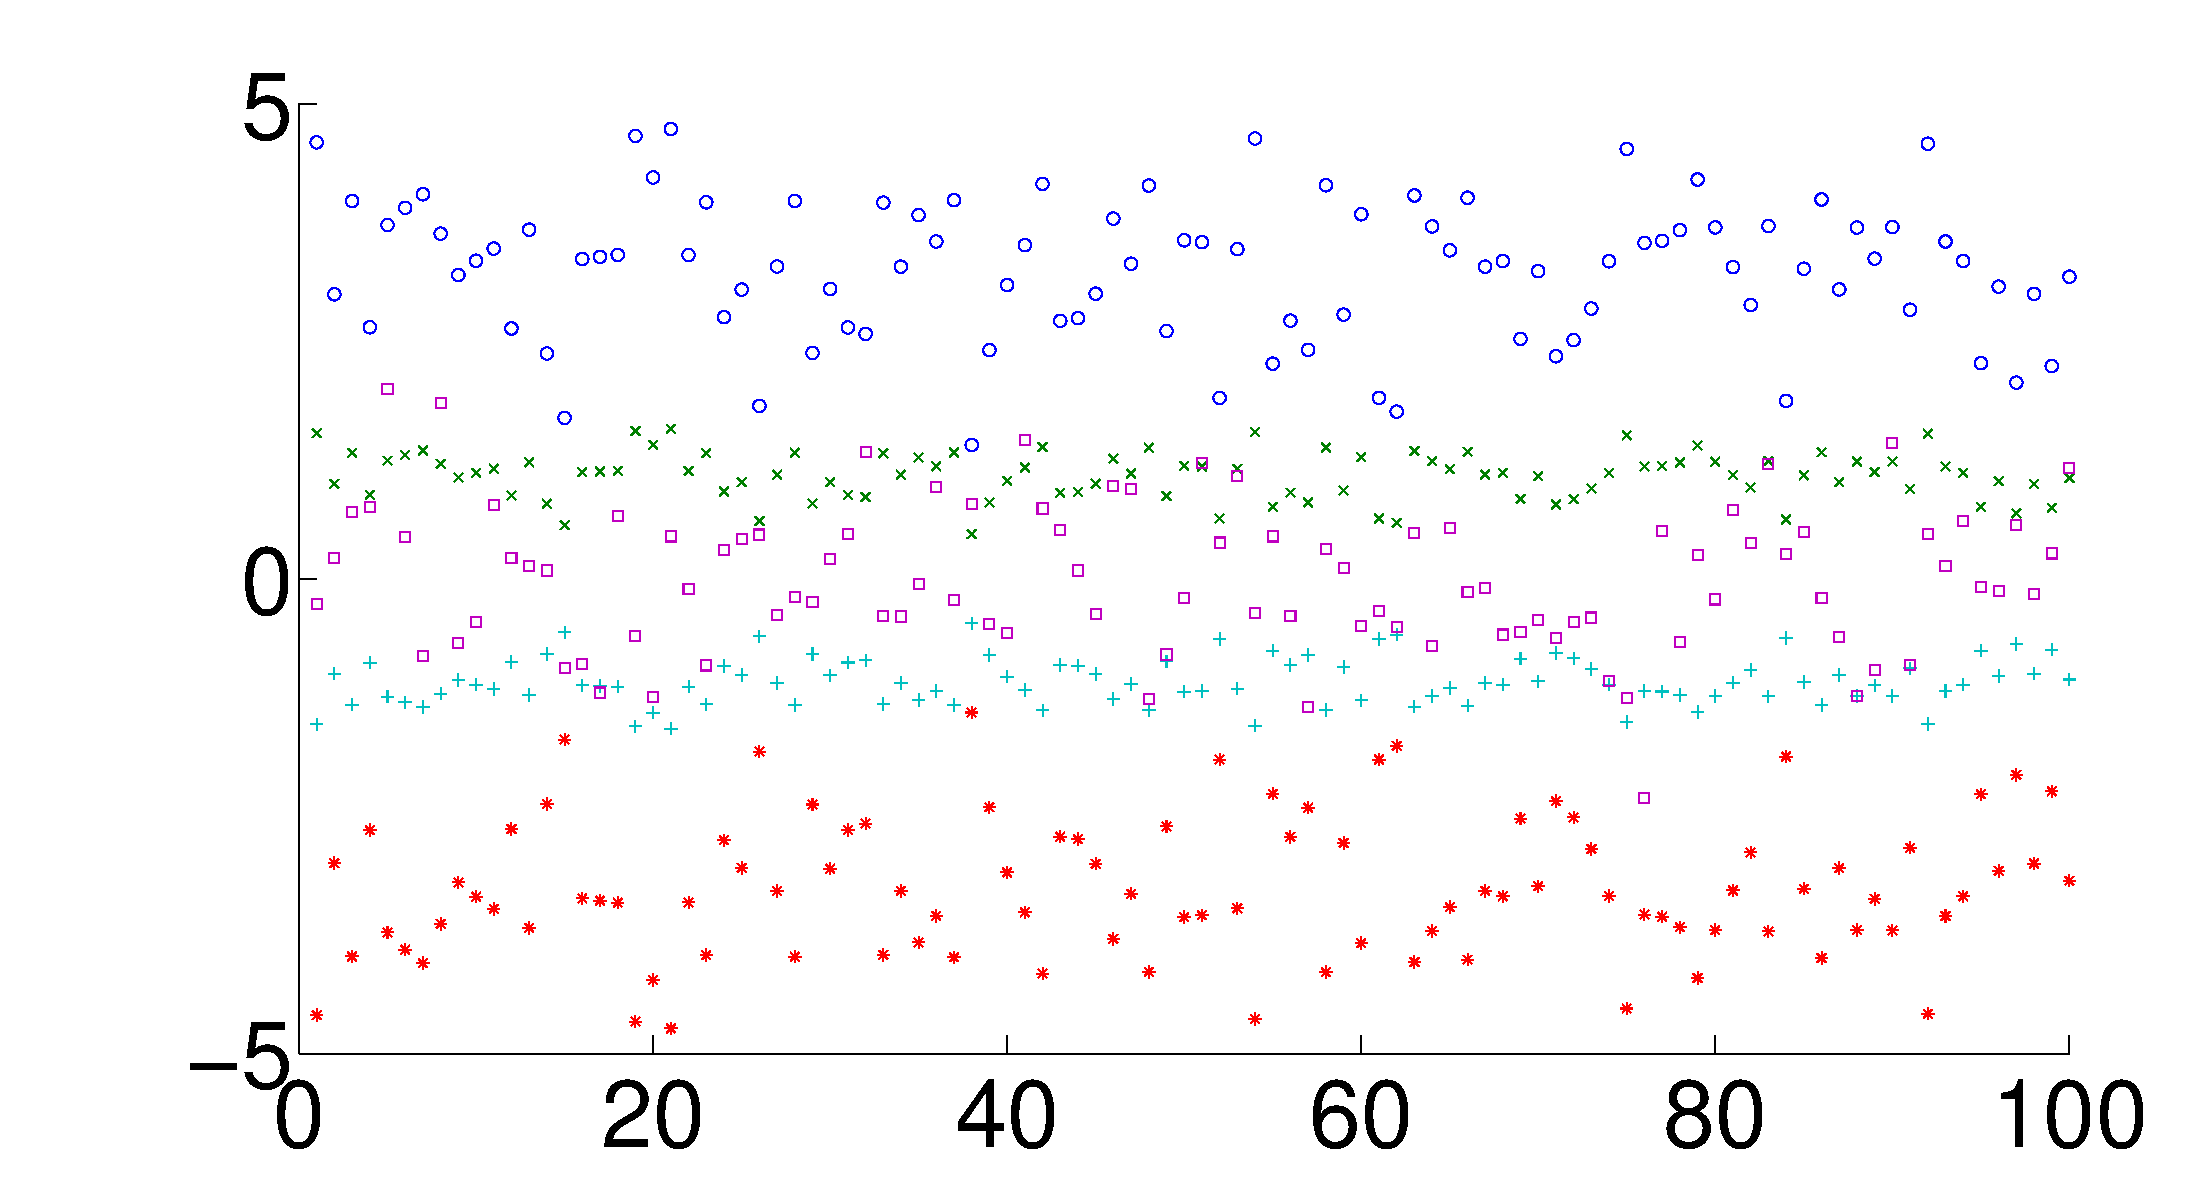
\includegraphics[scale=0.112]{fig/clusters.eps} &
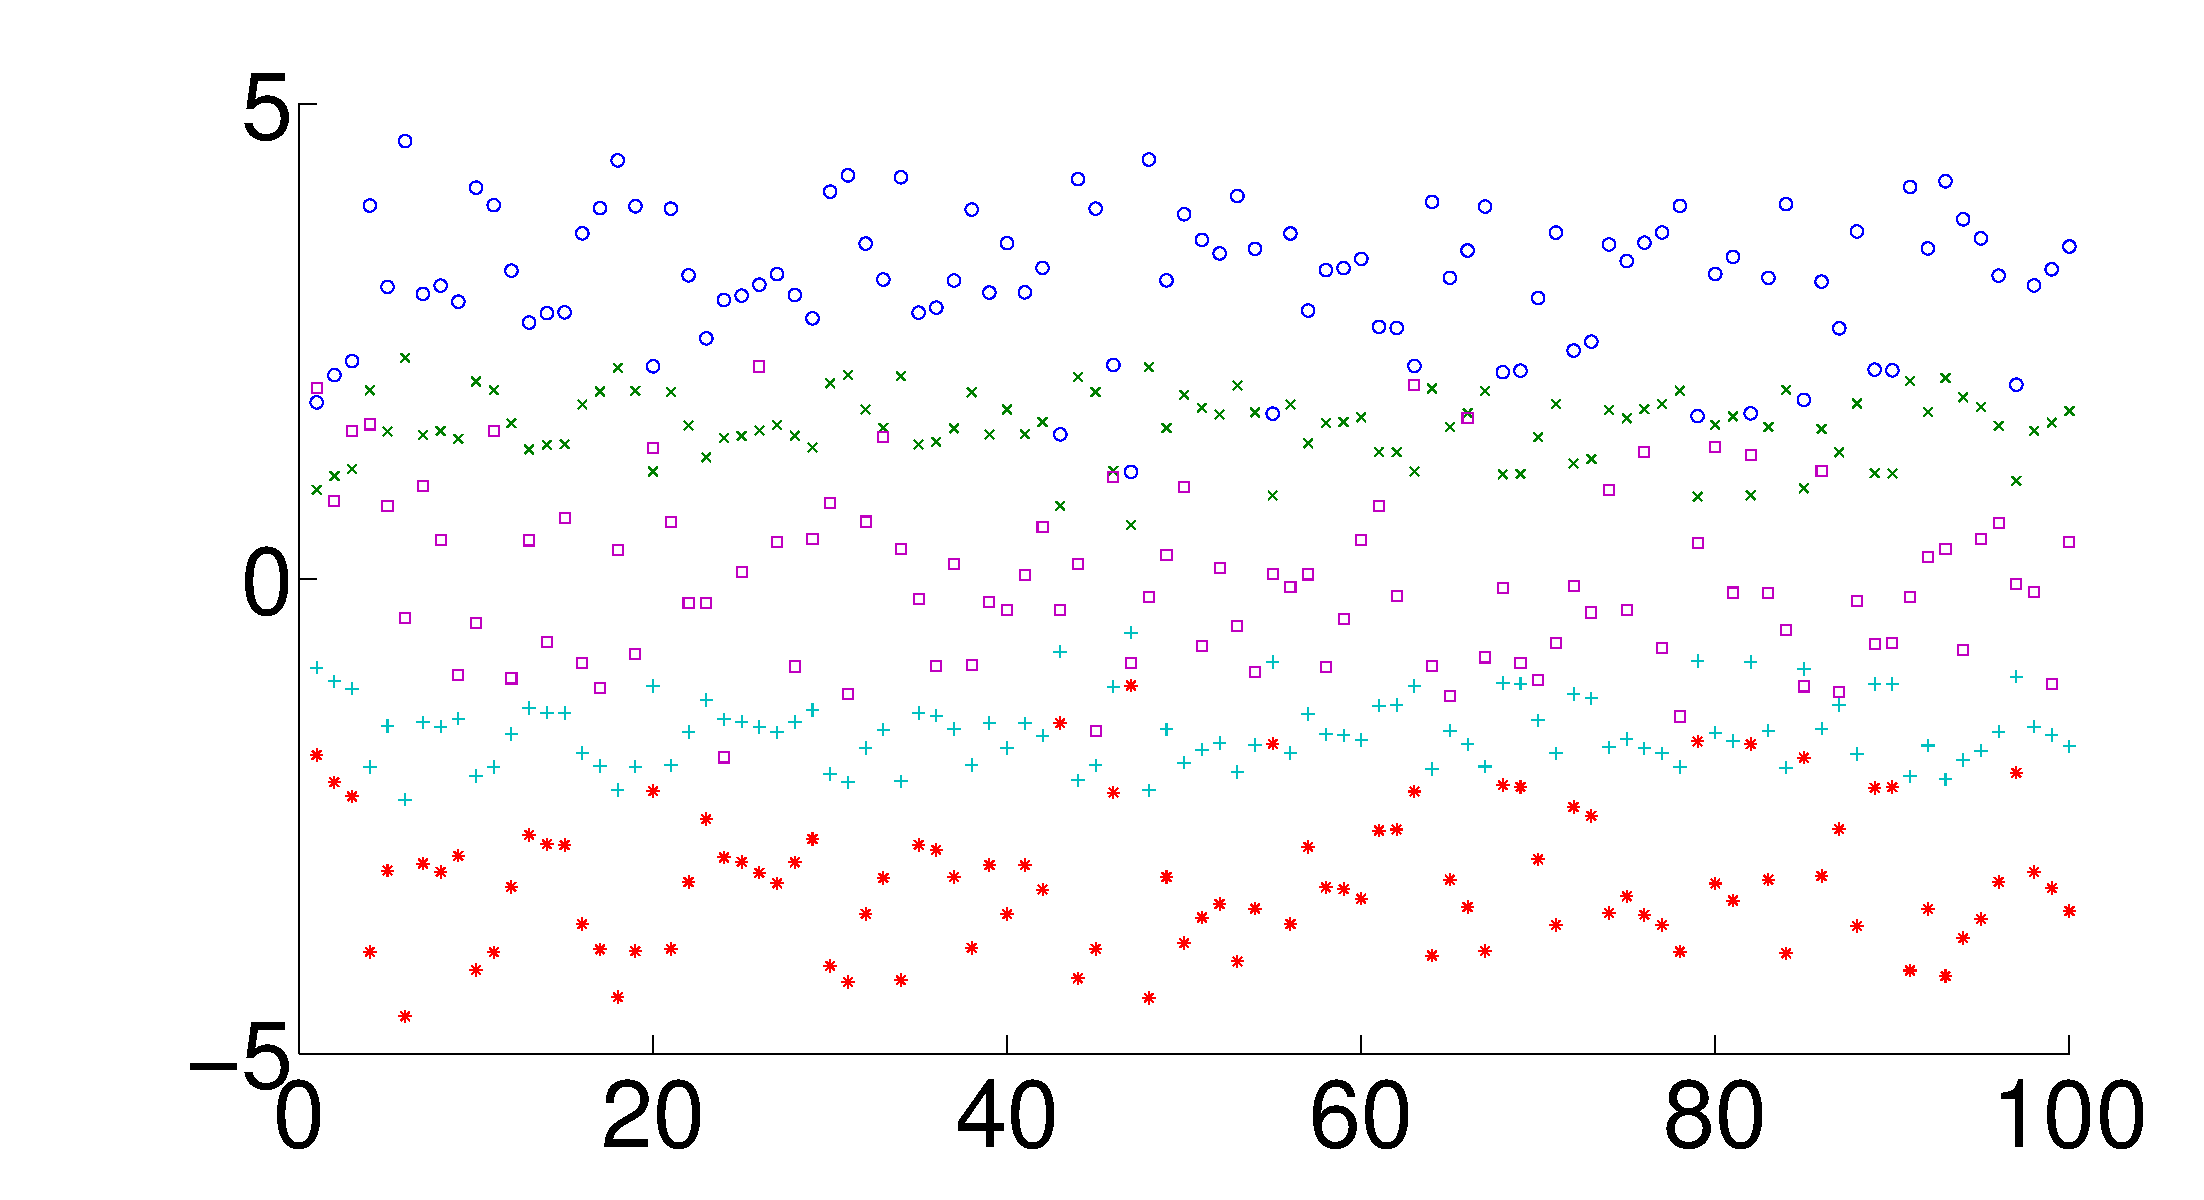
\includegraphics[scale=0.112]{fig/clusters4.eps} &
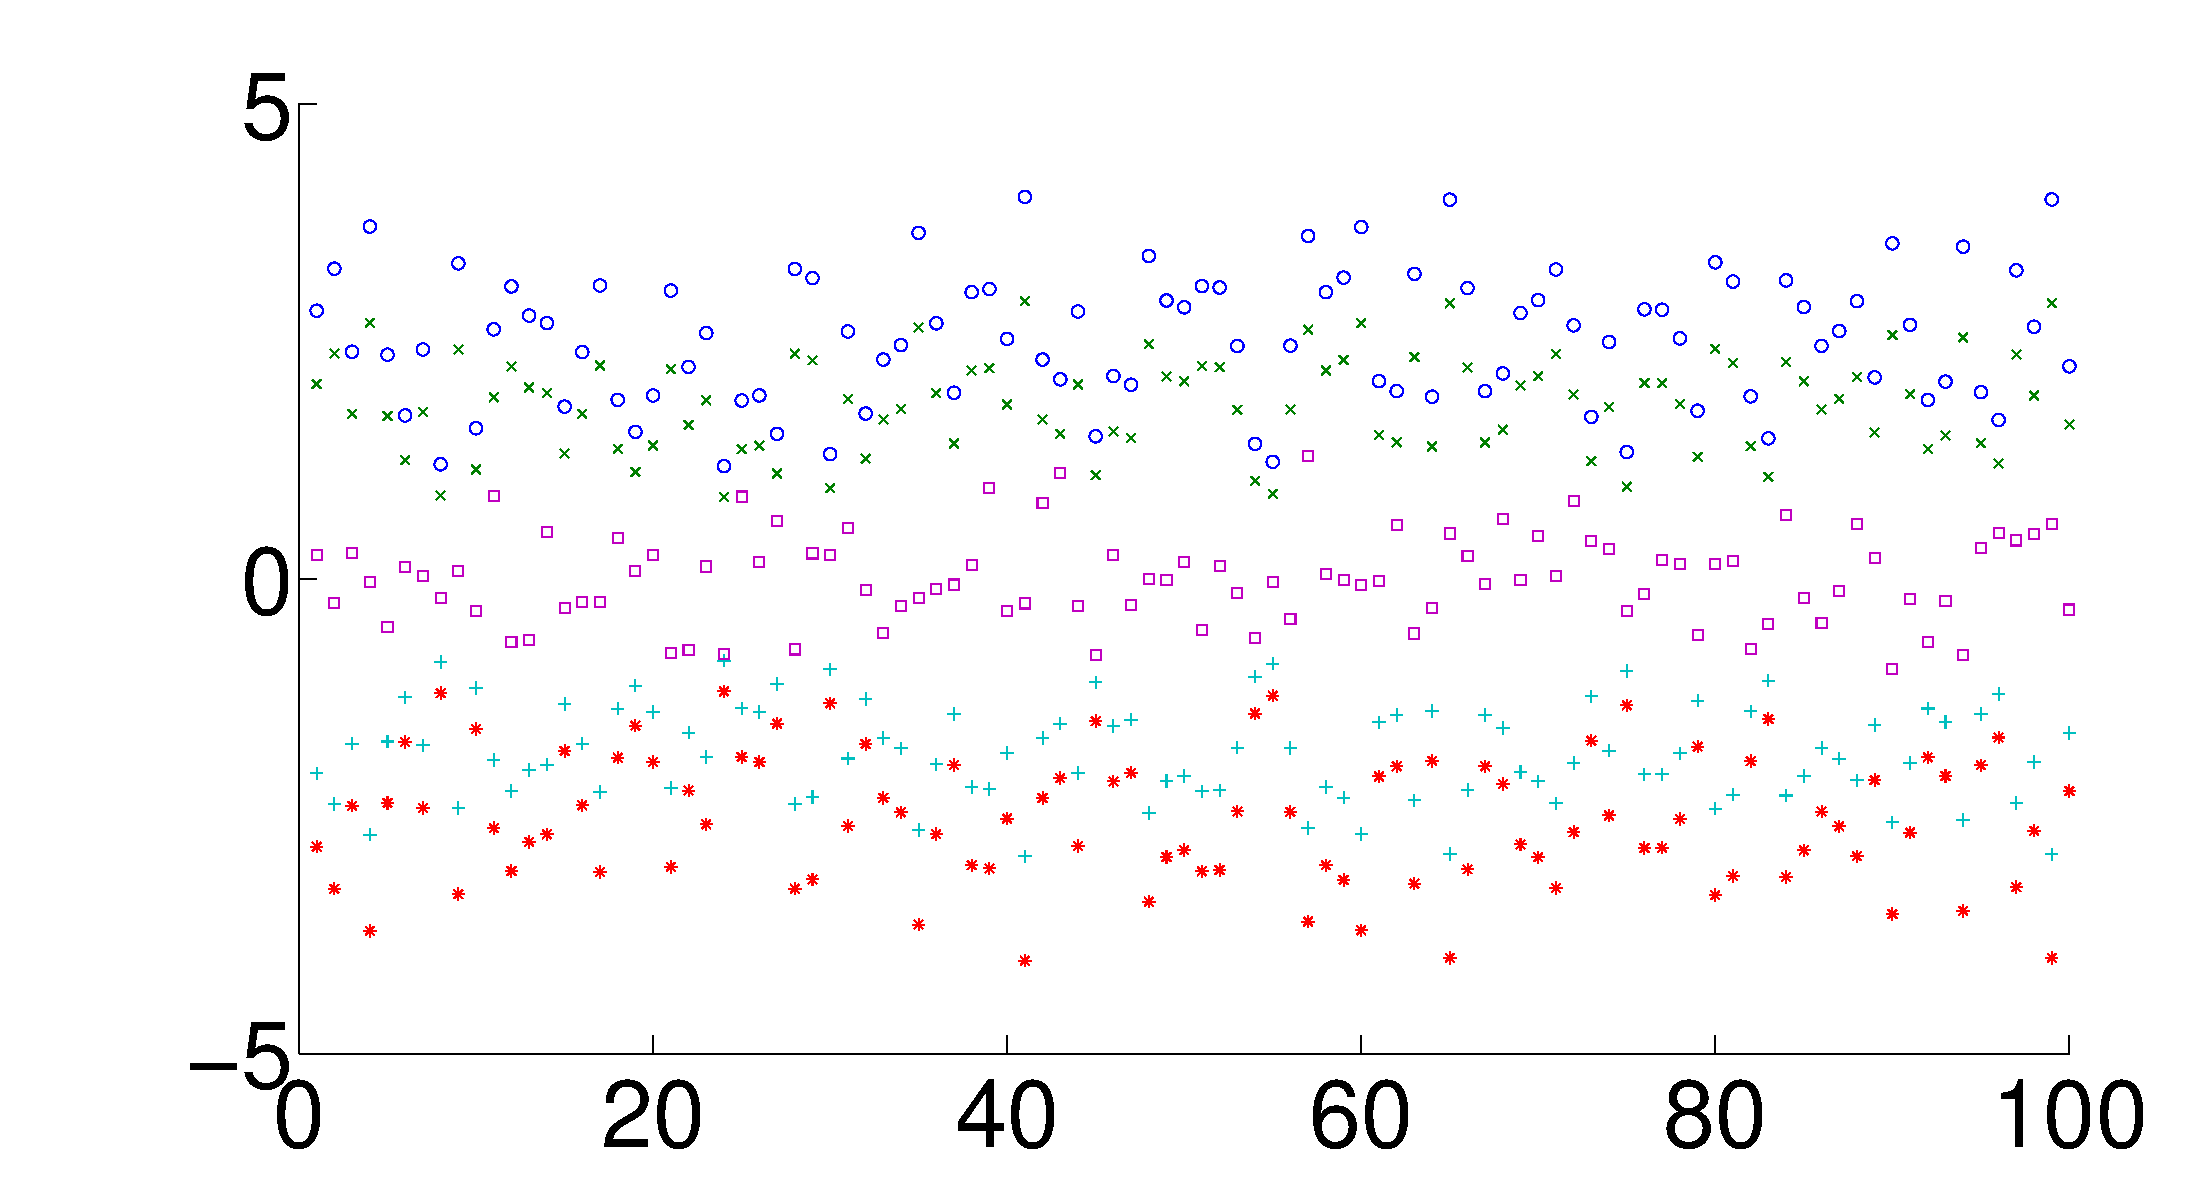
\includegraphics[scale=0.112]{fig/clusters3.eps} \\
$a_1$ --- range: [-4.74, 4.74] & $a_3$ --- range: [-4.61, 4.61] & $a_2$ --- range: [-4.02, 4.02] \\
$\mu$: 0, $\sigma$:2.26 &$\mu$: 0, $\sigma$:2.30 & $\mu$: 0, $\sigma$:2.18 \\
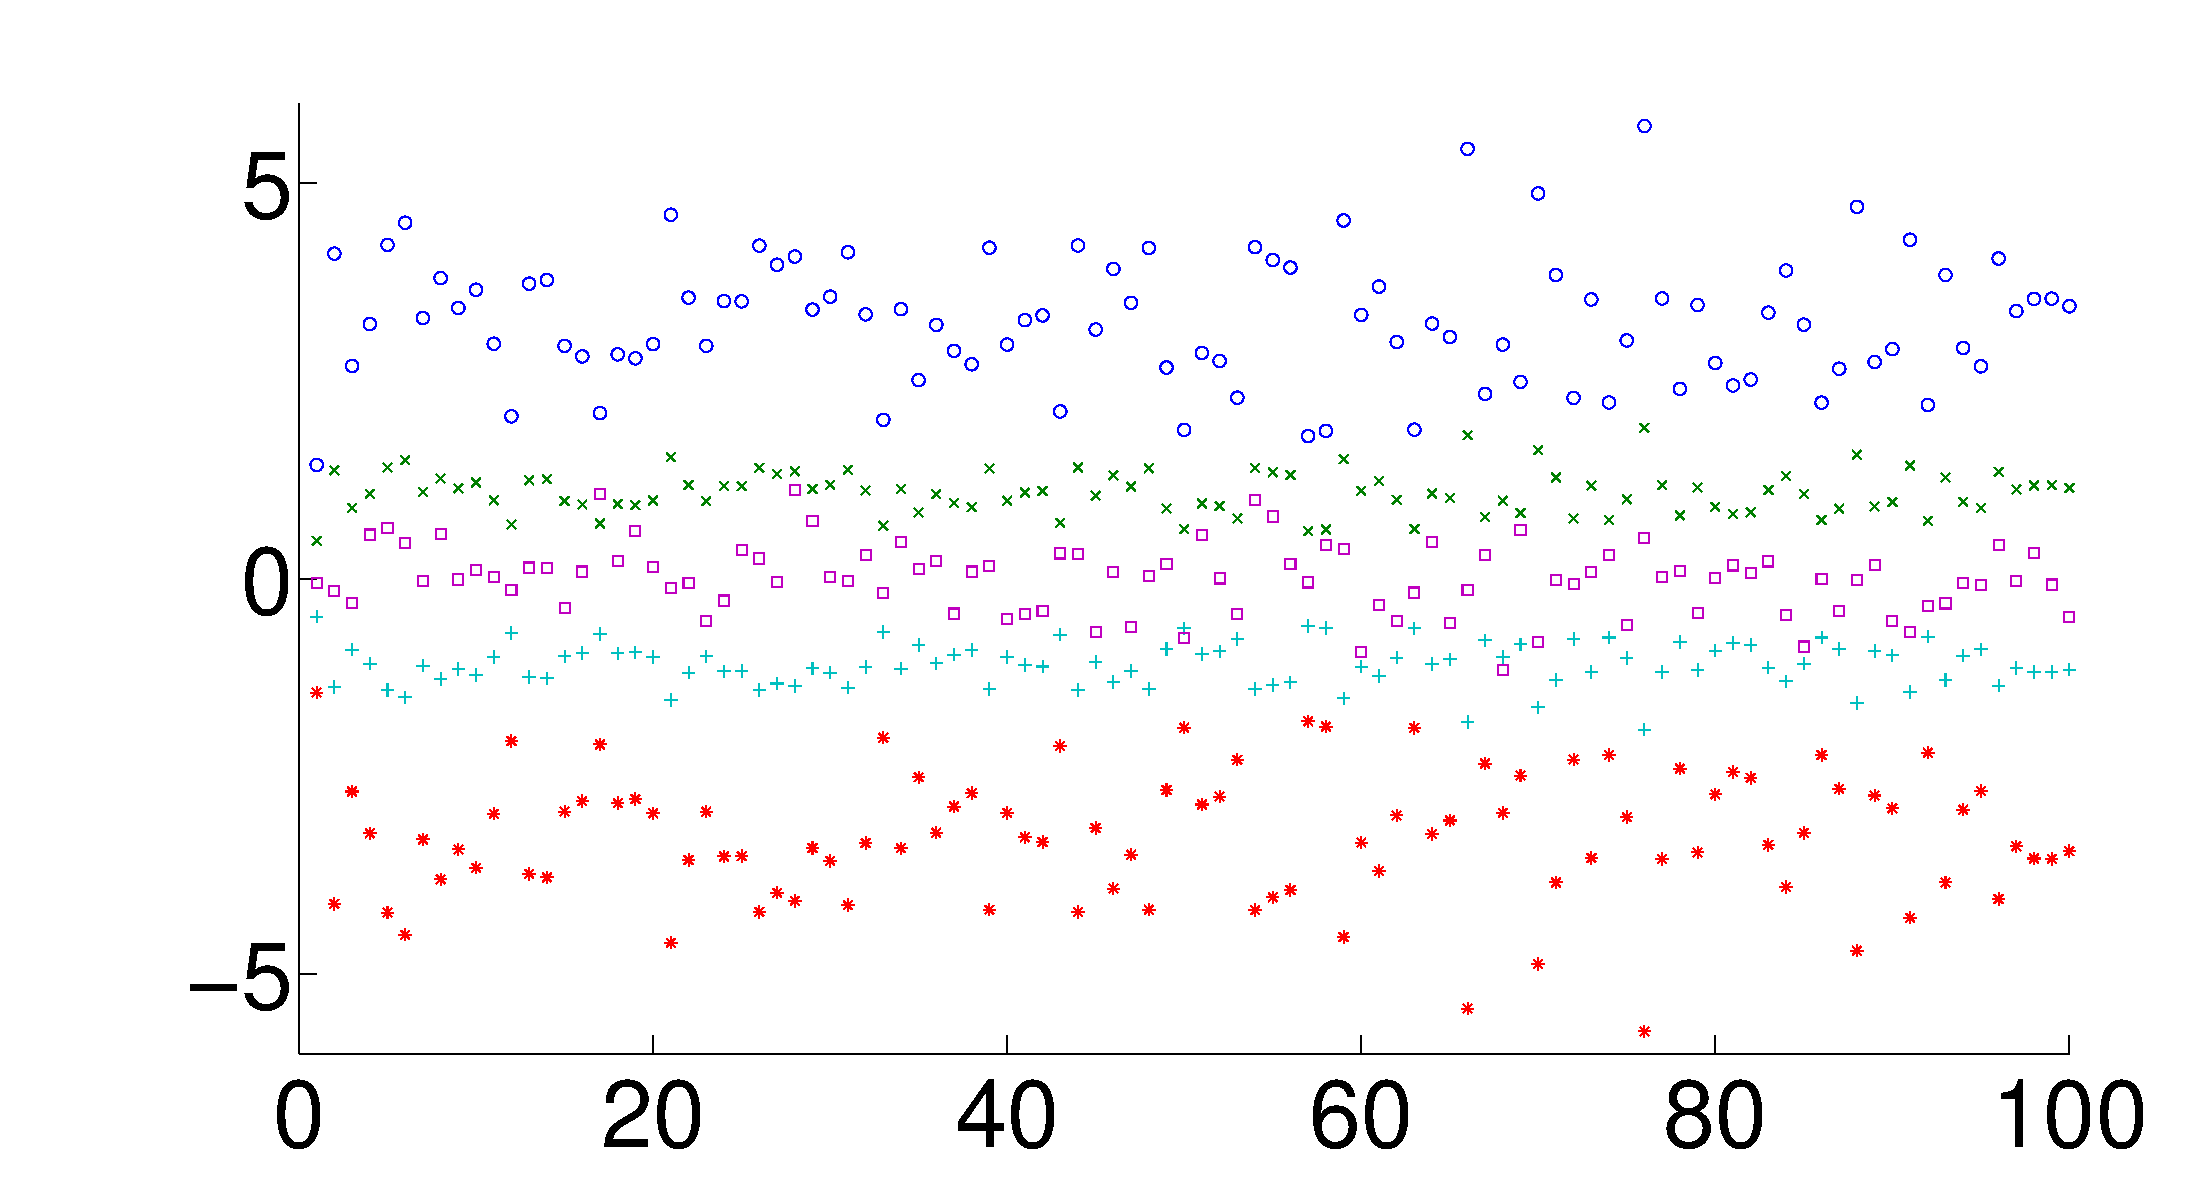
\includegraphics[scale=0.112]{fig/clusters21.eps} &
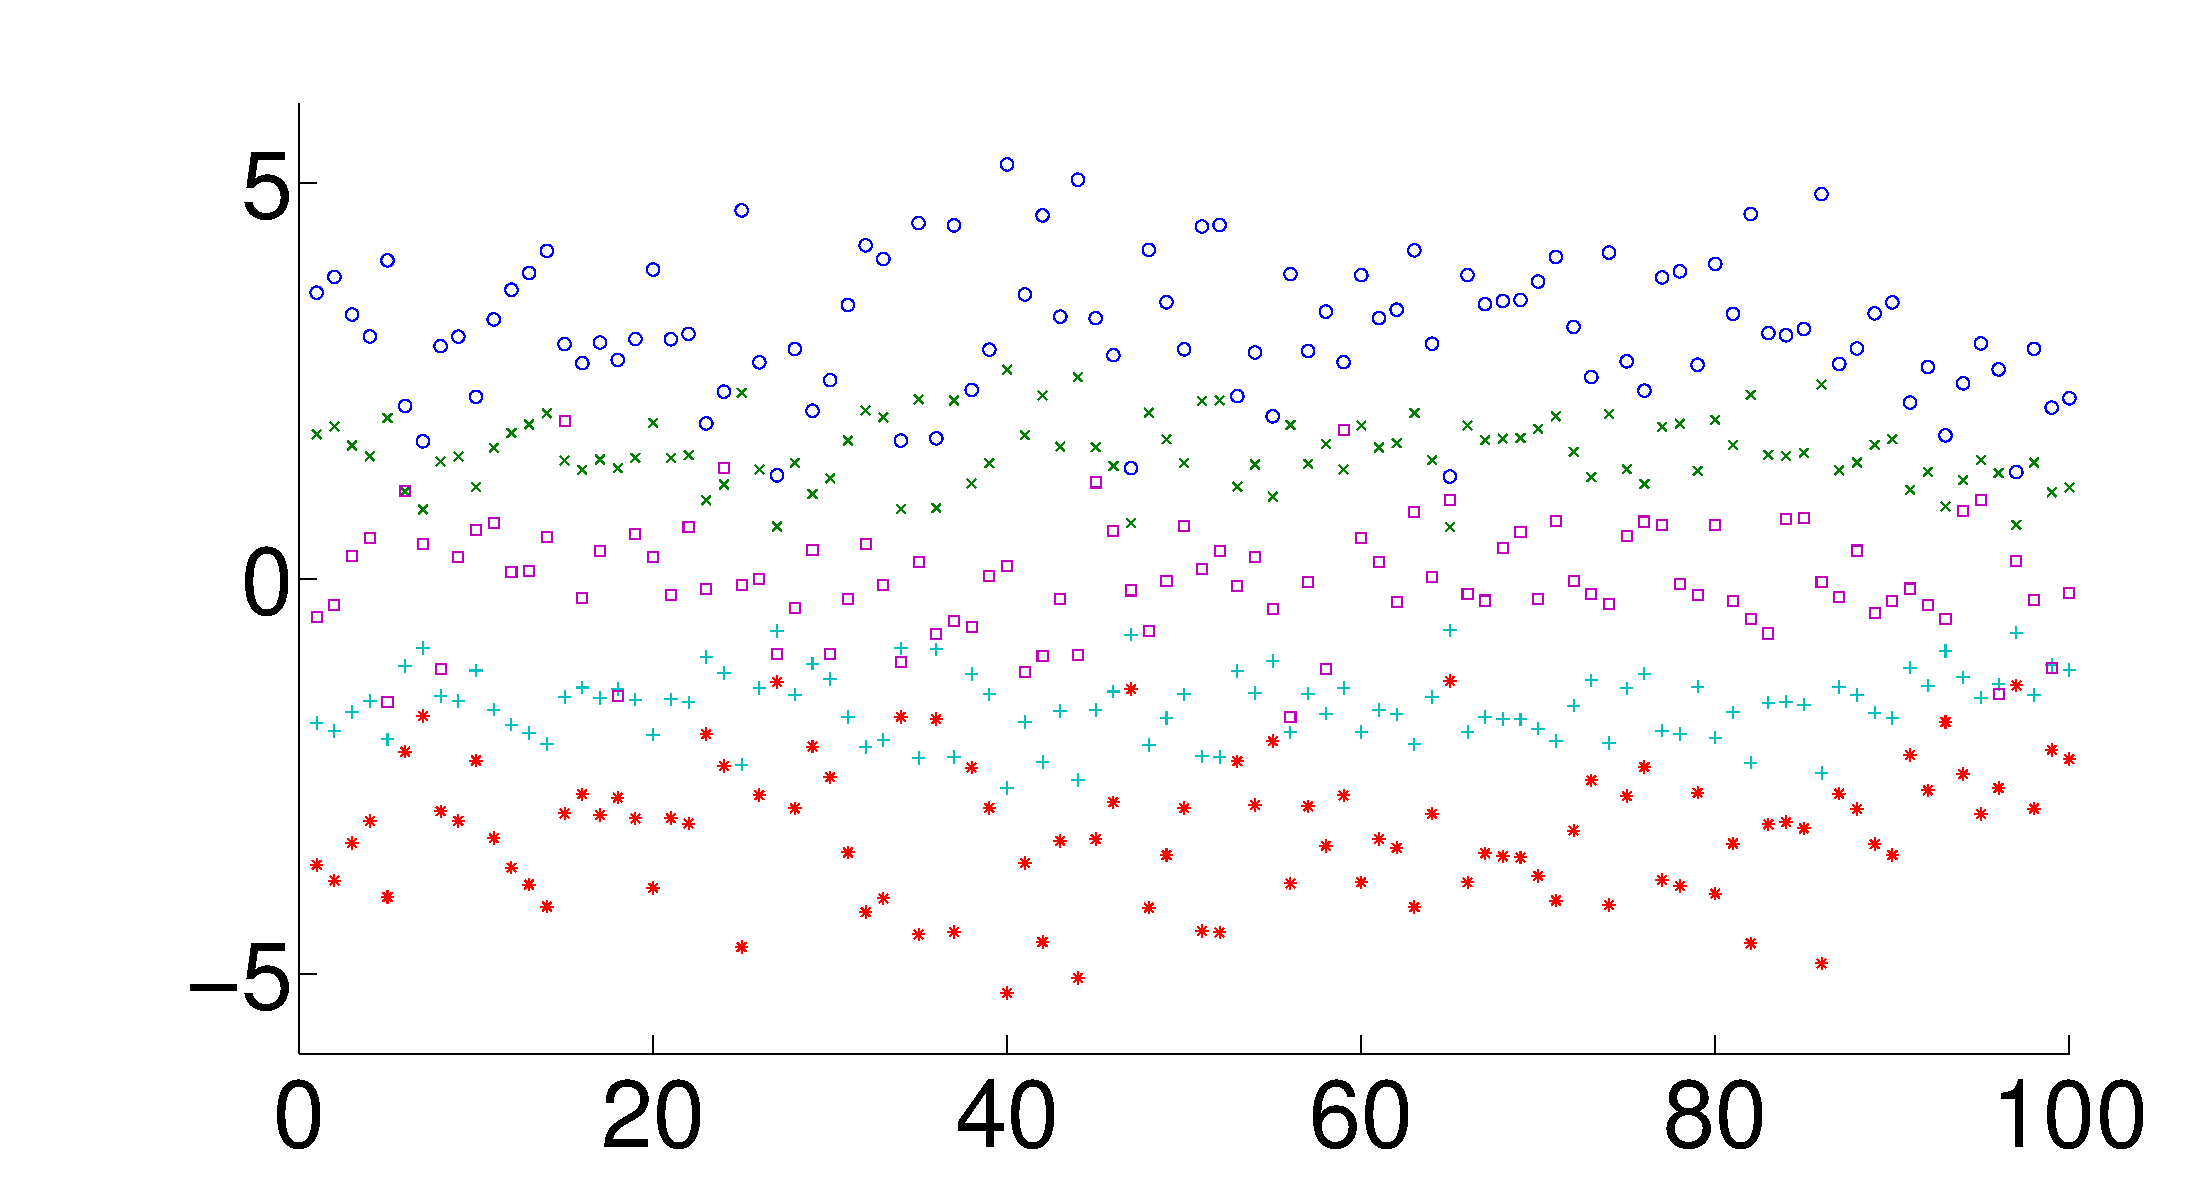
\includegraphics[scale=0.112]{fig/clusters23.eps} &
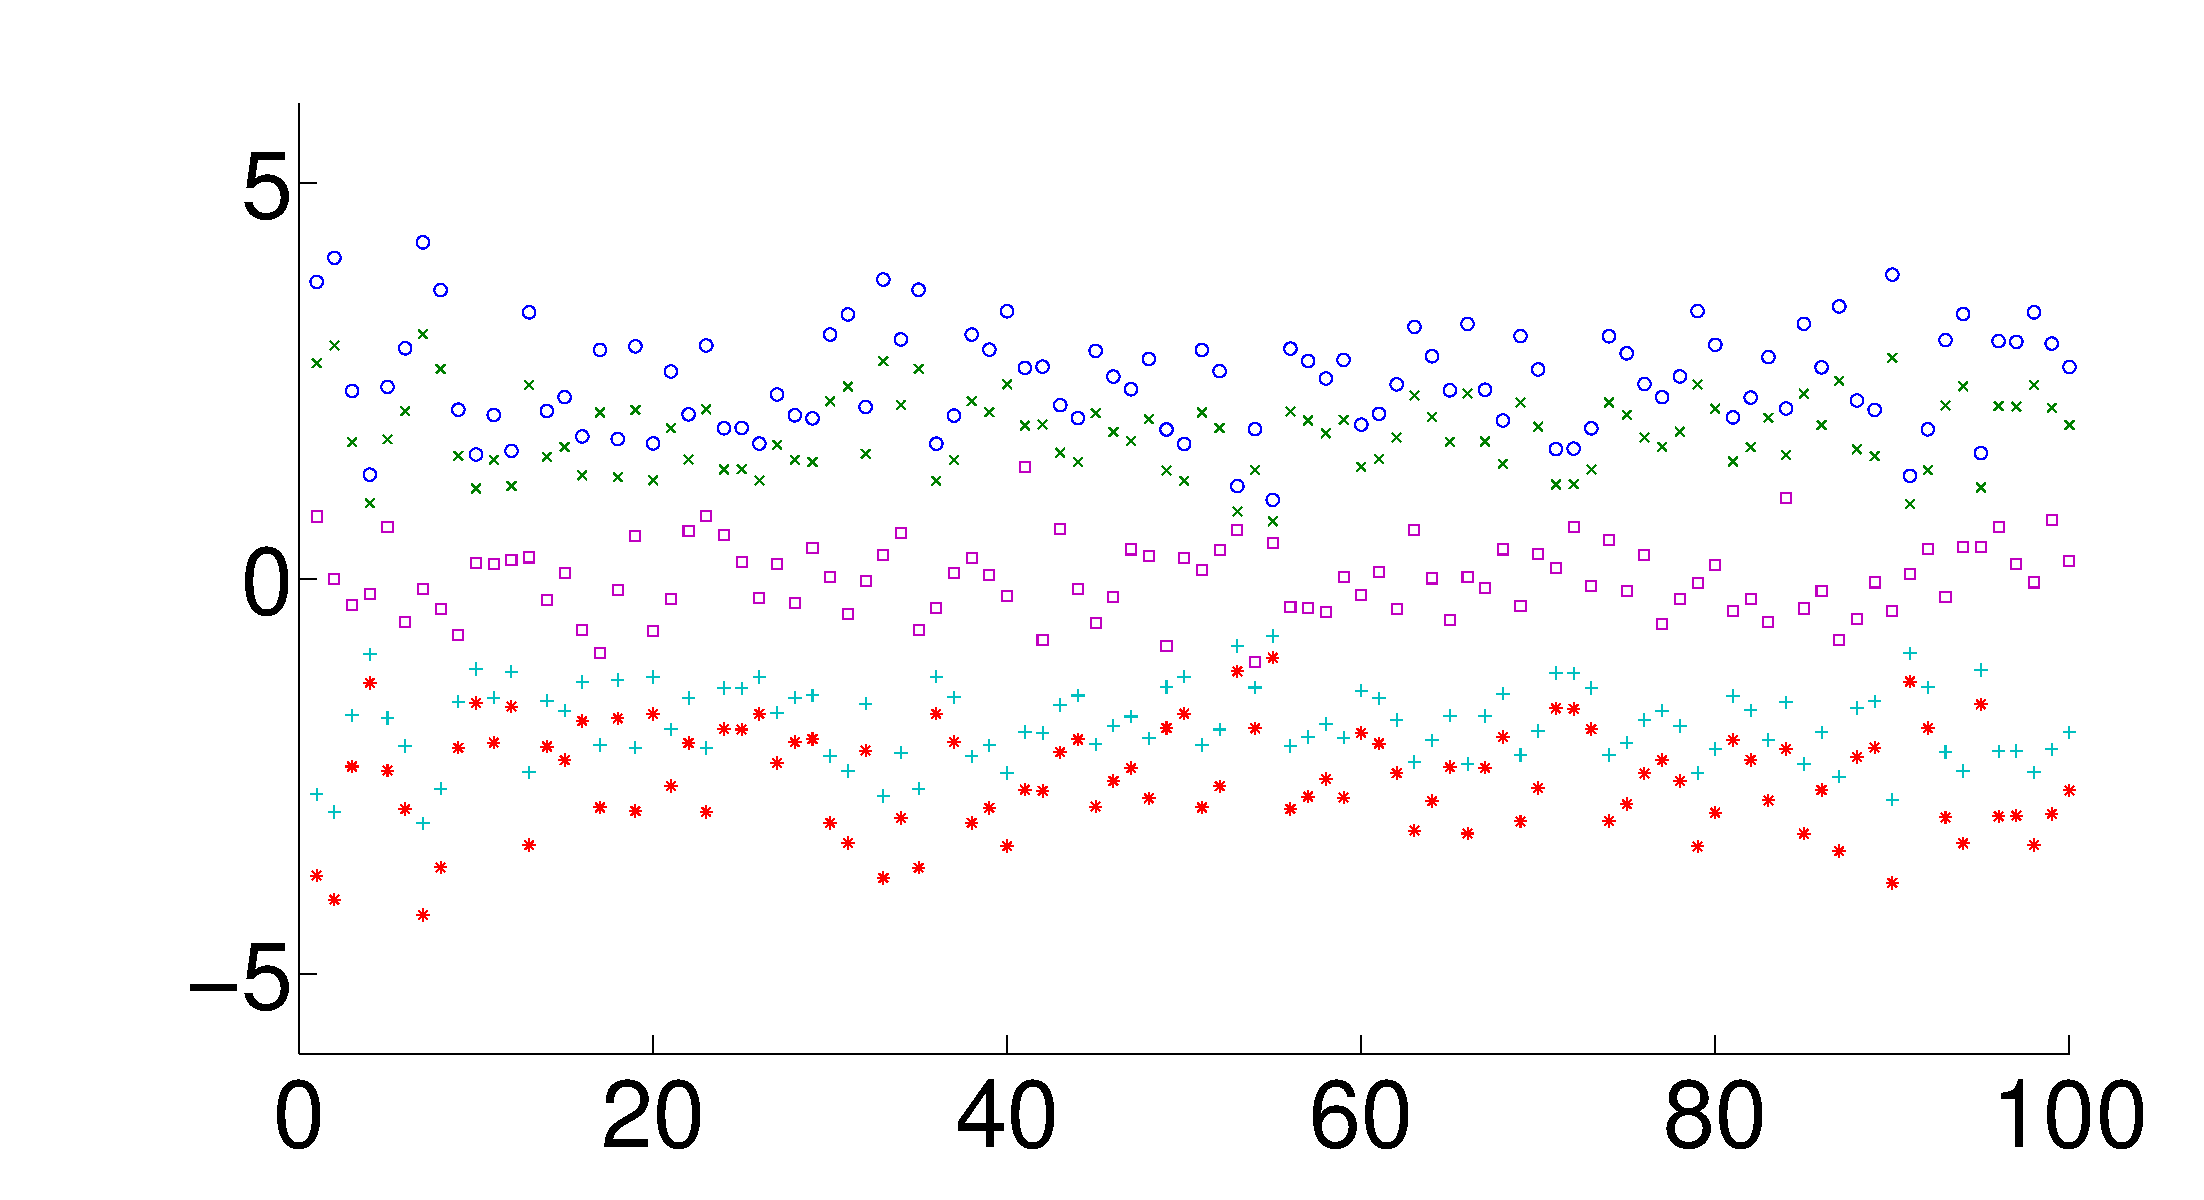
\includegraphics[scale=0.112]{fig/clusters22.eps} \\
$a_1'$ --- range: [-5.72, 5.72] & $a_3'$ --- range: [-5.24, 5.24] & $a_2'$ --- range: [-4.25, 4.25] \\
$\mu$: 0, $\sigma$:2.20 & $\mu$: 0, $\sigma$:2.35 & $\mu$: 0, $\sigma$:2.15 \\
\end{tabular}
\end{center}
\caption[Synthetic data generation.]{\label{fig:syndata} Scatter plots of data instances from three sample attributes in one synthetic dataset (upper frame) and those of their corresponding attributes from another (lower frame) are illustrated to show their respective value distributions.}
\end{figure*}

\subsubsection{Results:}
Figure~\ref{fig:syn_pareto} illustrates the Pareto front obtained from matching two synthetic datasets, each having 20 attributes and 5 clusters. Most notably, the gold standard results for both attribute matching and cluster matching are obtained from the left-most point on the Pareto front. In other words, given the decision variables ($X$) corresponding to that point, we obtained 100\% correct matching results. We further observed that in our subsequent tests on other synthetic datasets with varied number of attributes and clusters, the derived Pareto fronts all contain the gold standard result, and the point corresponding to the gold standard can always be found towards the minimum end of $f_a$. Given this, we propose the following method to reduce the Pareto-optimal set to a single point corresponding to the most favored choice ($X^*$) in the decision space. The idea is to find the decision with the minimum weighted sum of objective values in the obtained Pareto-optimal set, i.e., $X^*=\stackbin[X]{}{\argmin}~\big[\alpha f_a(X)+\beta f_c(X)\big]$, where $\alpha$ and $\beta$ are weights. We first conducted preliminary experiments to determine the best values for $\alpha$ and $\beta$ (0.8 and 0.2 respectively) and used them in all subsequent experiments. This method works markedly well on the synthetic datasets. For all the tests described in Table~\ref{tbl:scale}, 100\% correct results for both attribute and cluster matchings are obtained (hence we omit the precision in the table).
\begin{figure}[tb]
\begin{center}
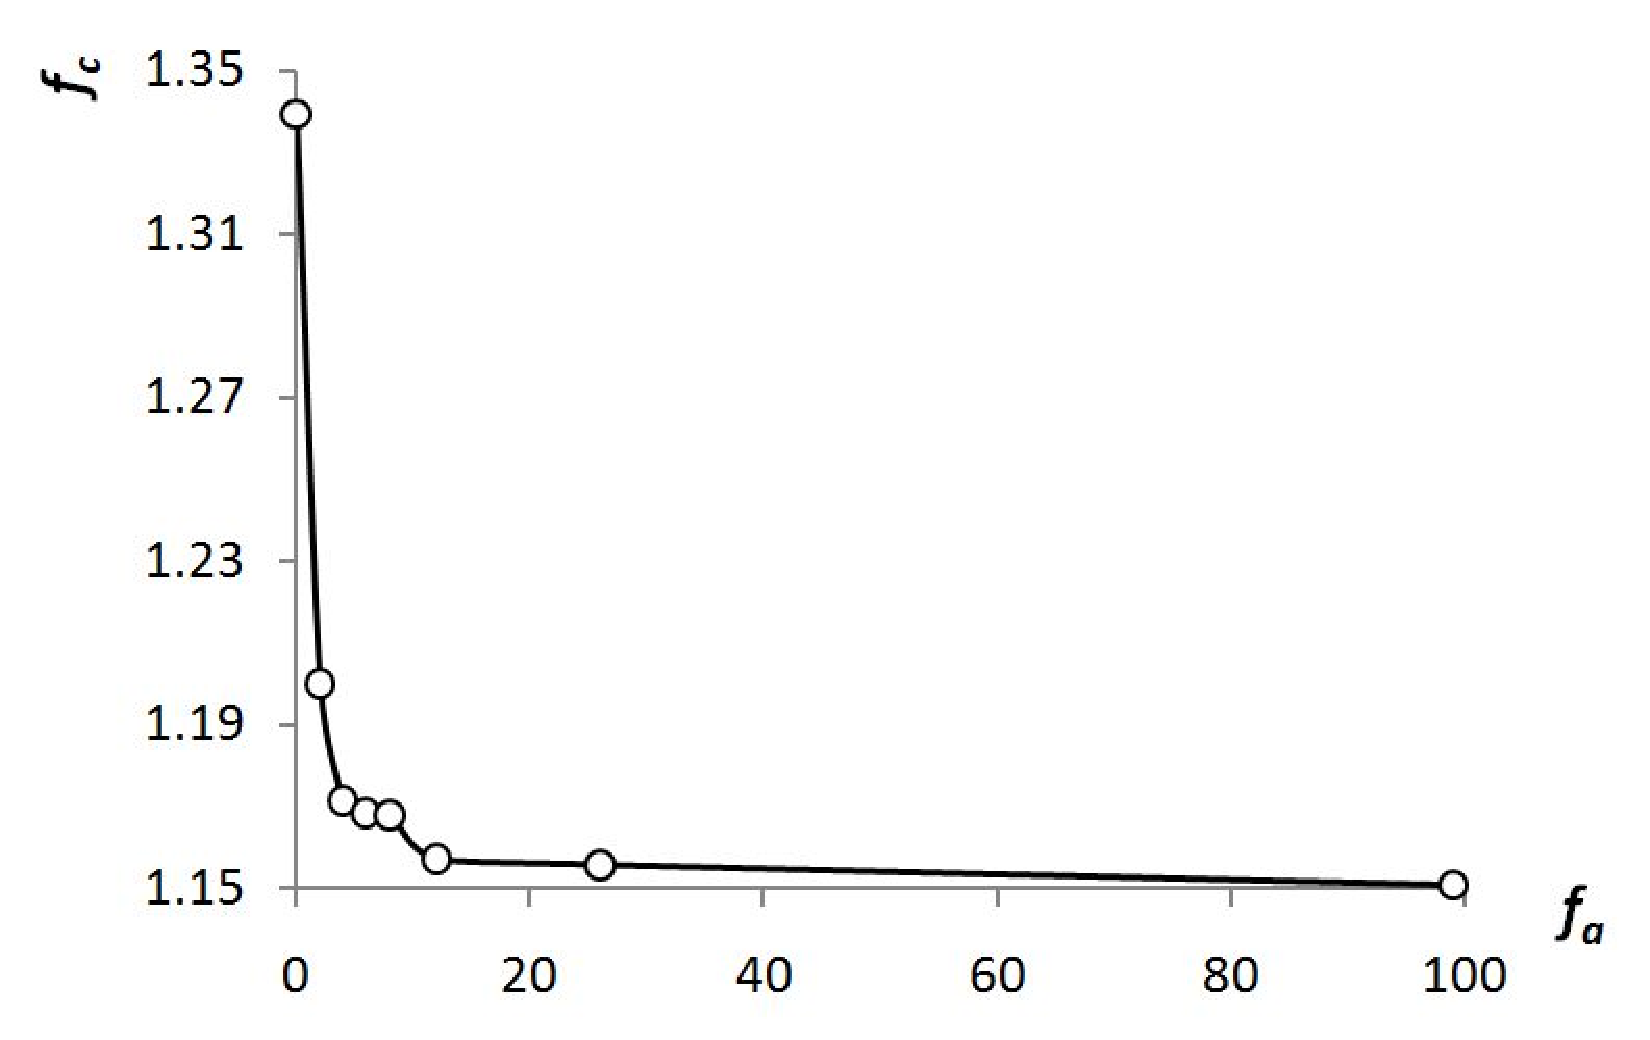
\includegraphics[width=0.4\textwidth]{fig/syn_pareto.eps}
\end{center}
\caption[An example Pareto front.]{\label{fig:syn_pareto} An example Pareto front obtained from matching two synthetic datasets with 20 attributes and 5 clusters.}
\end{figure}

\subsubsection{Running Time:}
We systematically altered the number of attributes and clusters present in the data and conducted a series of tests to show the scalability of the proposed method. The running time under different configurations is reported in Table~\ref{tbl:scale}. The time is calculated by averaging over 5 runs of each test (on a 2.53GHz dual-core CPU with 4 gigabytes memory), each run having 1000 iterations in the simulated annealing process. The main computationally expensive part of the annealing process is the generation of new candidate solution phase (function $G$) in which an assignment problem is solved using the Hungarian method. The complexity of the Hungarian method is cubic and is already the most efficient algorithm for solving the assignment problem (e.g., a brute force algorithm has a factorial complexity). Fortunately, rarely is the case that the number of attributes or clusters is large in real-world scenarios where the proposed technique is needed. For reasonable configurations in most practical applications, the computation time is within a tractable range as shown in table~\ref{tbl:scale}.
\begin{table}[tbh]
\begin{center}
\begin{tabular}{r|r|r}
\hline
\# attributes & \# clusters & time (sec)\\
\hline
5   &   20  &   0.28\\
20  &   20  &   1.81\\
20  &   40  &   7.04\\
20  &   60  &   17.80\\
40  &   20  &   4.66\\
40  &   40  &   11.74\\
40  &   60  &   25.93\\
60  &   20  &   10.95\\
60  &   40  &   20.70\\
60  &   60  &   37.35\\
100 &   100 &   172.23\\
\hline
\end{tabular}
\end{center}
\caption[Running time.]{\label{tbl:scale} Running time of the annealing process on synthetic datasets with varied configurations of attribute and cluster sizes. The time is obtained by averaging over results of 5 runs of each test.}
\end{table}

\subsection{Neuroscience Dataset}
\subsubsection{Data Acquisition:}
%The difficulty is especially pronounced in many scientific domains where there have been an increasing interest in nationwide and worldwide inter-institute collaboration. An example of such collaborative project is research in experimental event-related brain potential (ERP) analysis carried out at the NEMO (Neural Electromagnetic Ontologies) consortium laboratories. The heterogeneity among participating groups hinders meaningful meta-analysis despite the large number of studies in the field.

To address the problems of attribute and cluster matching in a real-world neuroscience application, we used a set of realistic simulated ERP (event-related potentials) datasets, which were designed to support evaluation of ERP analysis methods~\cite{FrishkoffEtal07}. The datasets were specifically designed to simulate heterogeneous data from different groups of subjects under different conditions (via distinct simulated brain activities), as well as distinct measurement methods (spatial and temporal metrics) and distinct patterns (reflecting two different pattern decomposition techniques). Real ERP data arise from superposition of latent scalp-surface electrophysiological patterns, each reflecting the activity of a distinct cortical network that cannot be reconstructed from the scalp-measured data with any certainty. Thus, real ERP data are not appropriate for evaluation of ERP pattern mapping. By contrast, simulated ERP data are derived from known source patterns and therefore provide the necessary gold standard for evaluation of our proposed methods.

The raw data for this study consist of 80 simulated event-related potentials (ERPs), in which each ERP comprises simulated measurement data for a particular subject ($n$ = 40). The 40 simulated subjects are randomly divided into two 20-subject groups, SG1 and SG2, each containing 40 ERPs (20 subjects in 2 experimental conditions). Each ERP consists of a superposition of 5 latent varying spatiotemporal patterns. These patterns were extracted from the two datasets, SG1 and SG2, using two techniques: temporal Principal Components Analysis (tPCA) and spatial Independent Components Analysis (sICA), two data decomposition techniques widely used in ERP research~\cite{Dien2010}. To quantify the spatiotemporal characteristics of the extracted patterns, two alternative metric sets, m1 and m2, were applied to the two tPCA and the two sICA derived datasets. For a complete explanation of these alternative metrics, please see Appendix in~\cite{FrishkoffEtal07}.

In summary, the simulated ERP data generation process yielded eight test datasets in total, reflecting a 2 (attribute sets) $\times$ 2 (subject groups) $\times$ 2 (decomposition methods) factorial design. Therefore, for each attribute sets there are 4 datasets generated from different combinations of subject groups and decomposition methods, resulting $4 \times 4 = 16$ cases for the studies of attribute matching and cluster matching. The reason to include such variabilities was to test the robustness of our matching method to different sources of heterogeneities across the different datasets. Within all test datasets, 5 major ERP spatiotemporal patterns are present. They are P100, N100, N3, MFN, and P300. These patterns can be identified in the datasets by clustering analysis. Pretending that the latent patterns underlying discovered clusters are unknown, we hope to match clusters across datasets to recover the fact that the same patterns are present in all datasets.

\subsubsection{Results:}
%Figure~\ref{fig:nemo_exp} illustrates the Pareto fronts derived by the proposed method on each of the 16 test cases.
We applied the weighted sum method as the post-process step after obtaining the Pareto-optimal solutions to determine the most favored choice using the parameters ($\alpha$ and $\beta$) discovered in the preliminary experiments on synthetic datasets (cf. Section~\ref{sec:syn_exp}). The accuracy of attribute matching and cluster matching along with the number of points in the Pareto front are listed in Table~\ref{tbl:nemo_perf} (all these results are obtained by taking average from 5 runs for each test case).

%\begin{figure*}[tb]
%\begin{center}
%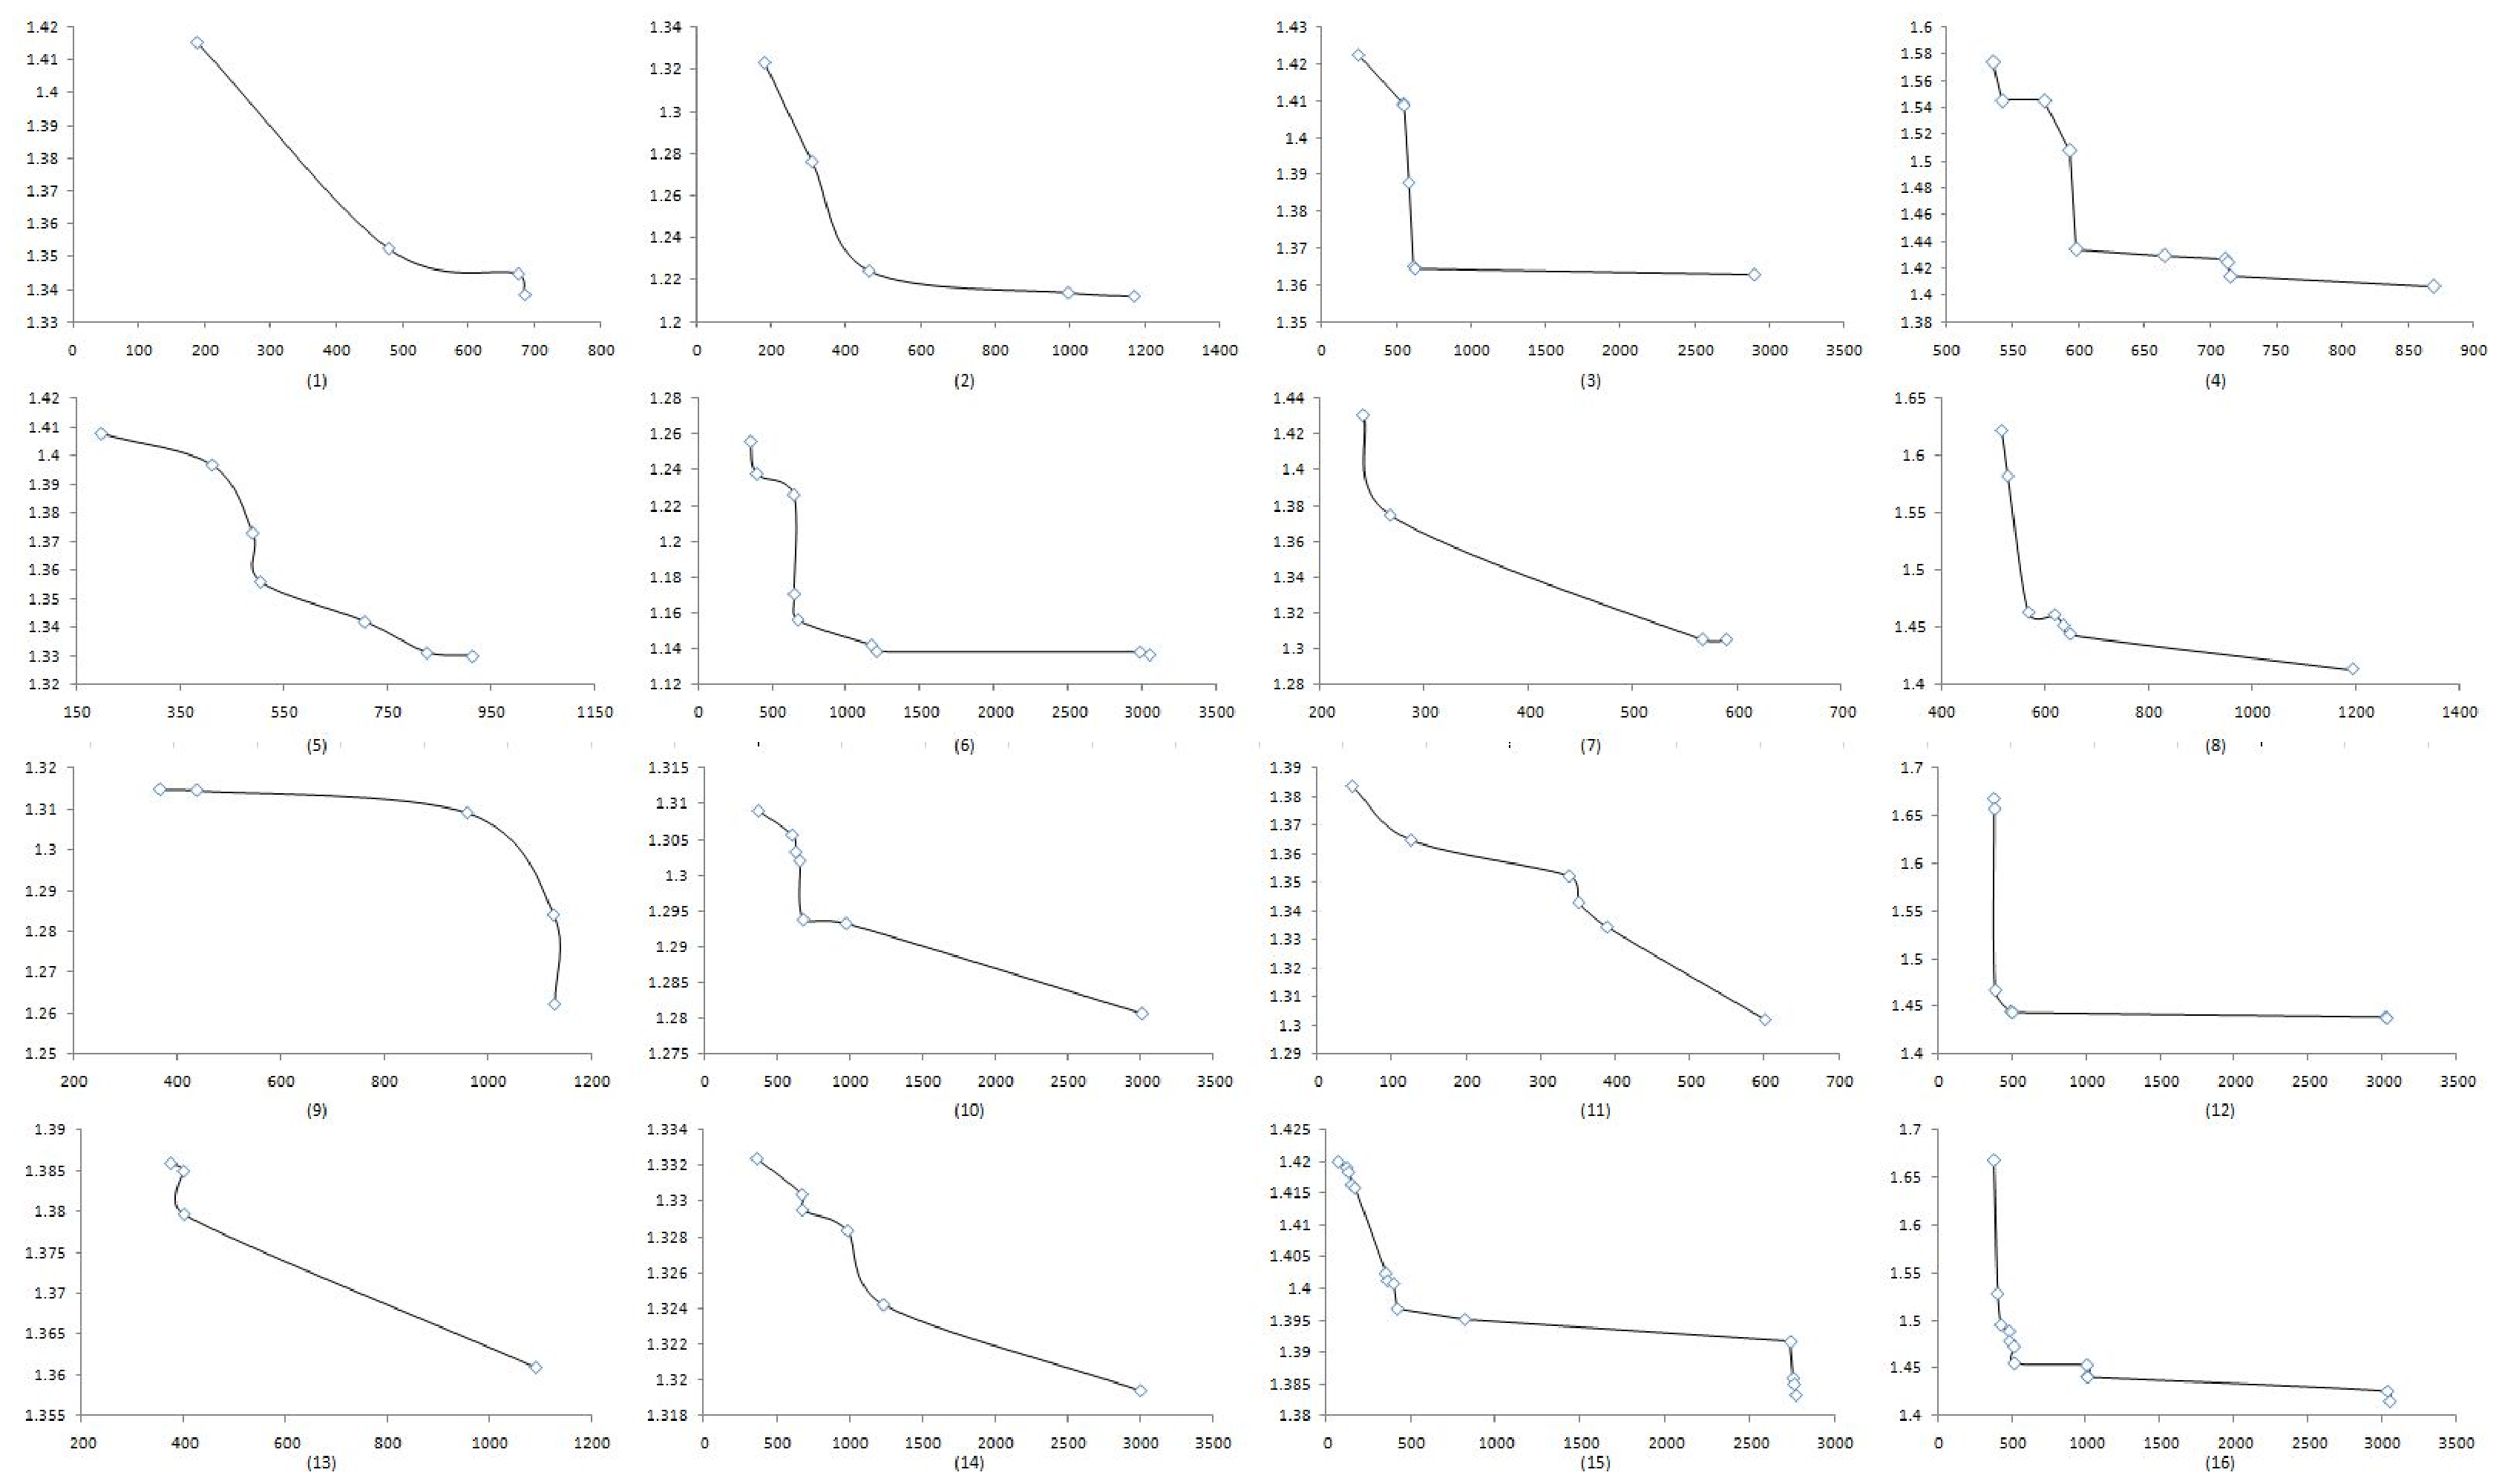
\includegraphics[width=1.\textwidth]{nemo_exp2.eps}
%\end{center}
%\caption{\label{fig:nemo_exp} Pareto fronts obtained from the 16 test cases of the neuroscience dataset.}
%\end{figure*}

It can be observed from the results in Table~\ref{tbl:nemo_perf} that more different factors involved in the acquisition of the two datasets for matching can negatively affect the matching performance. For example, in test case 1, the two datasets are drawn from the same subject group (SG1) and preprocessed using the same decomposition method (sICA); whereas in test case 4, the subject groups and decomposition methods are all different, resulting in greater variability and hence the performance is less satisfactory.

It is worth noting that our method greatly outperforms a baseline method called WS (see Figure~\ref{fig:perf_comp}) that determines attribute matching based on data distribution at the whole attribute level, which is typical in previous systems such as SemInt~\cite{Li00semint:a}. In this figure we also demonstrate the accuracy of the segmented statistics characterization with expert-labeled patterns, meaning that the data is partitioned and aligned in the most accurate way, which marks the best achievable attribute matching performance. But it is not feasible because, as mentioned in~Section~\ref{sec:intro}, manually recognizing patterns (partitioning data) and aligning them across datasets requires a priori knowledge of attributes in the datasets which is exactly what the problem of attribute matching tries to discover (the circular causality problem). On the other hand, our method does not require human involvement (except the specification of the number of clusters (patterns) present in the data in order to run the clustering analysis) in determining both the attribute matching and cluster matching and is able to achieve close-to-optimal results.

\begin{figure*}[tb]
\begin{center}
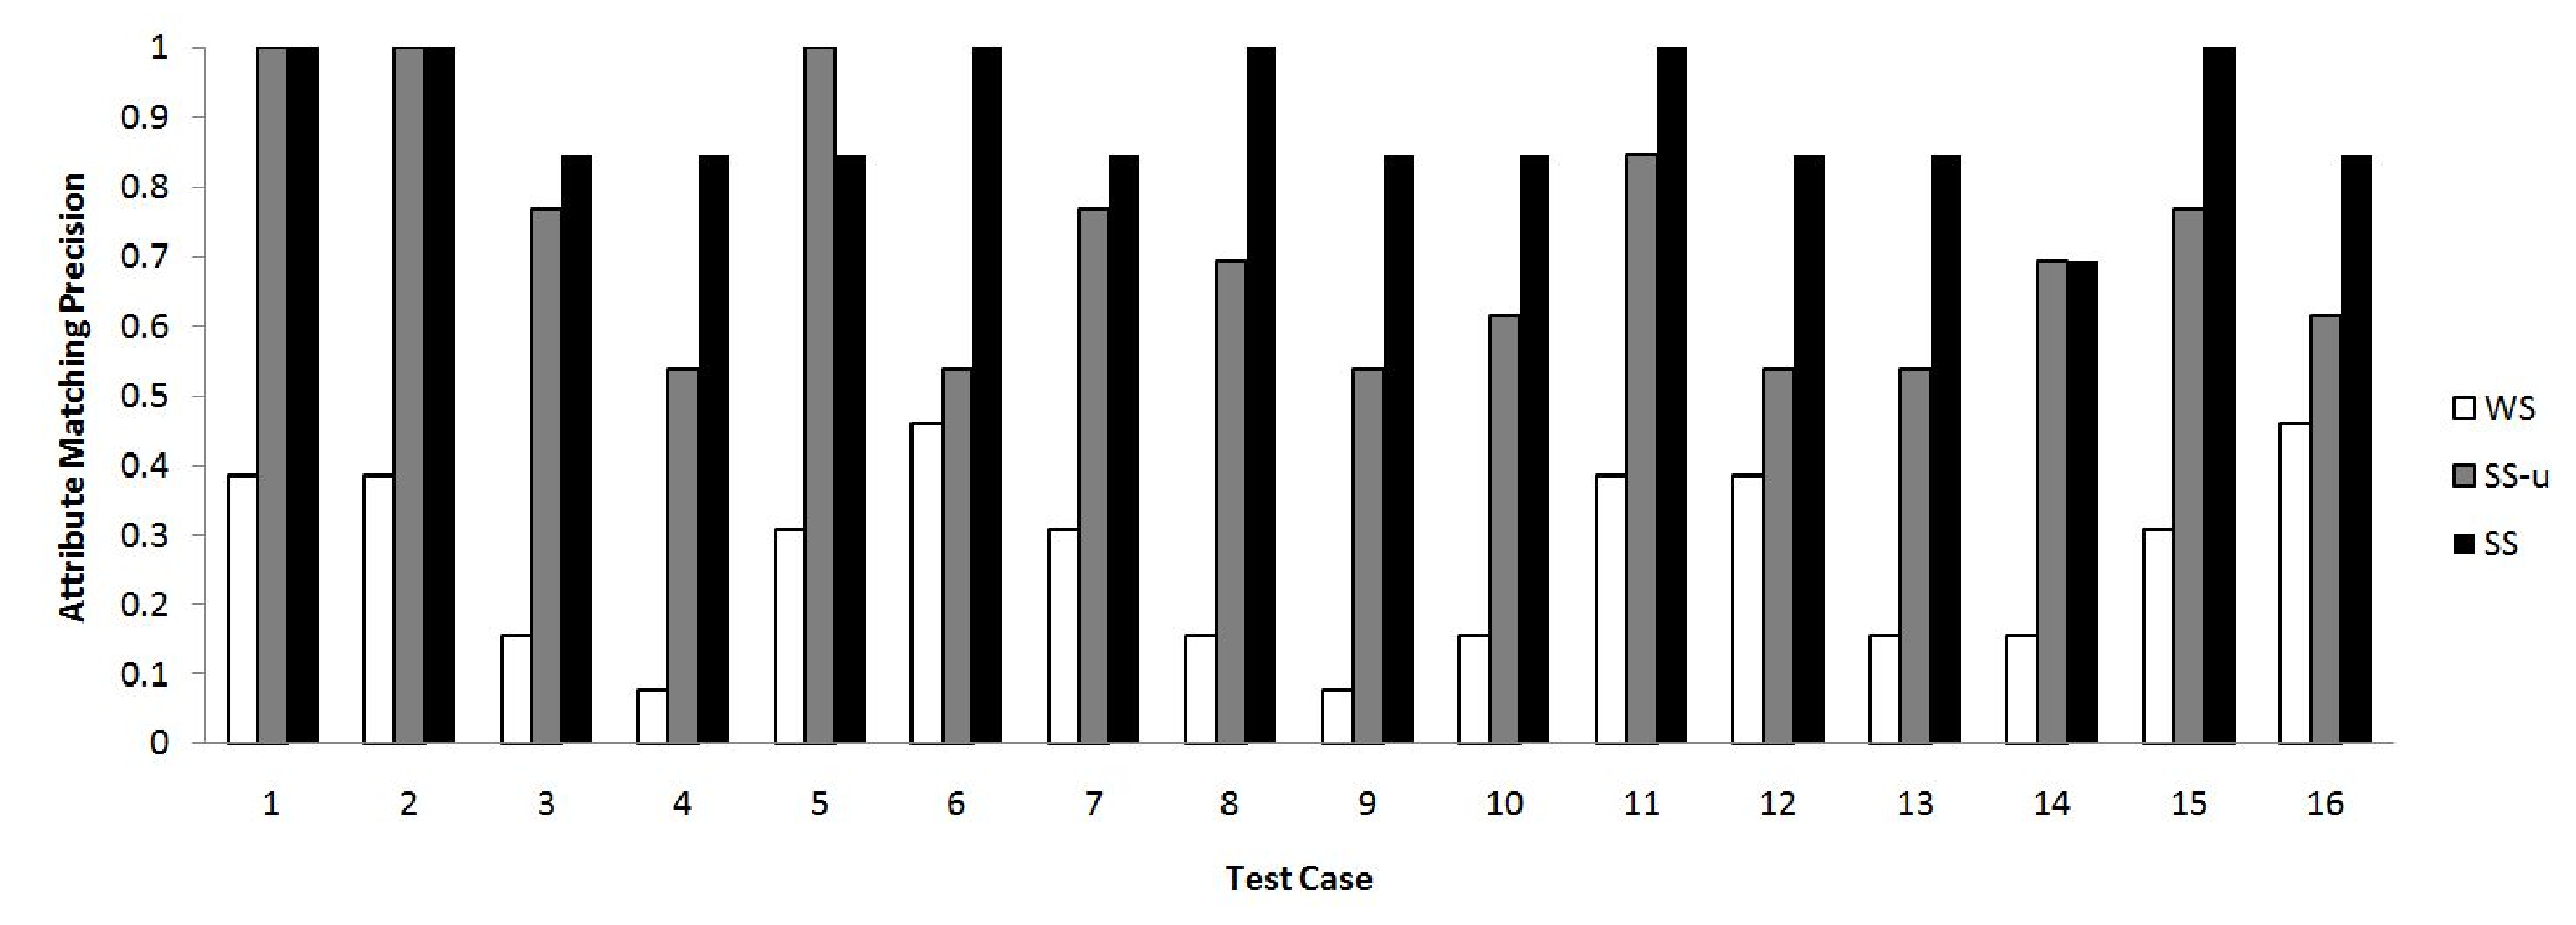
\includegraphics[width=1.\textwidth]{fig/perf_comp.eps}
\end{center}
\caption[Performance of MOSA on the neuroscience dataset.]{\label{fig:perf_comp} A comparison of the attribute matching accuracy of three methods on the 16 test cases of the neuroscience dataset. The three methods being compared are matching based on whole-attribute statistics (WS), segmented attribute statistics without knowing a priori cluster matching (SS-u), and segmented attribute statistics with expert-aligned clusterings (SS).}
\end{figure*}


\begin{table*}[tbh]
\begin{center}
\begin{tabular}{l|l|l|l|l|l}
\hline
Test case & Source params & Target params & $~~~P_a~~~$ & $~~~P_c~~~$ & $|\Sigma|$\\
\hline
1		&	$\langle$	SG1, sICA, m1	$\rangle$	&	$\langle$	SG1, sICA, m2	$\rangle$	&		13/13	&	5/5	&	5	 \\
2		&	$\langle$	SG1, sICA, m1	$\rangle$	&	$\langle$	SG2, sICA, m2	$\rangle$	&		13/13	&	5/5	&	6	 \\
3		&	$\langle$	SG1, sICA, m1	$\rangle$	&	$\langle$	SG1, tPCA, m2	$\rangle$	&		10/13	&	5/5	&	6	 \\
4		&	$\langle$	SG1, sICA, m1	$\rangle$	&	$\langle$	SG2, tPCA, m2	$\rangle$	&		7/13	&	3/5	&	8	 \\
5		&	$\langle$	SG2, sICA, m1	$\rangle$	&	$\langle$	SG1, sICA, m2	$\rangle$	&		11/13	&	3/5	&	7	 \\
6		&	$\langle$	SG2, sICA, m1	$\rangle$	&	$\langle$	SG2, sICA, m2	$\rangle$	&		13/13	&	5/5	&	7	 \\
7		&	$\langle$	SG2, sICA, m1	$\rangle$	&	$\langle$	SG1, tPCA, m2	$\rangle$	&		10/13	&	5/5	&	6	 \\
8		&	$\langle$	SG2, sICA, m1	$\rangle$	&	$\langle$	SG2, tPCA, m2	$\rangle$	&		9/13	&	2/5	&	8	 \\
9		&	$\langle$	SG1, tPCA, m1	$\rangle$	&	$\langle$	SG1, sICA, m2	$\rangle$	&		7/13	&	5/5	&	4	 \\
10		&	$\langle$	SG1, tPCA, m1	$\rangle$	&	$\langle$	SG2, sICA, m2	$\rangle$	&		8/13	&	5/5	&	6	 \\
11		&	$\langle$	SG1, tPCA, m1	$\rangle$	&	$\langle$	SG1, tPCA, m2	$\rangle$	&		11/13	&	5/5	&	6	 \\
12		&	$\langle$	SG1, tPCA, m1	$\rangle$	&	$\langle$	SG2, tPCA, m2	$\rangle$	&		7/13	&	3/5	&	5	 \\
13		&	$\langle$	SG2, tPCA, m1	$\rangle$	&	$\langle$	SG1, sICA, m2	$\rangle$	&		7/13	&	3/5	&	5	 \\
14		&	$\langle$	SG2, tPCA, m1	$\rangle$	&	$\langle$	SG2, sICA, m2	$\rangle$	&		9/13	&	5/5	&	6	 \\
15		&	$\langle$	SG2, tPCA, m1	$\rangle$	&	$\langle$	SG1, tPCA, m2	$\rangle$	&		10/13	&	3/5	&	8	 \\
16		&	$\langle$	SG2, tPCA, m1	$\rangle$	&	$\langle$	SG2, tPCA, m2	$\rangle$	&		8/13	&	3/5	&	8	 \\
\hline
\end{tabular}
\end{center}
\caption[A comparison between MOSA and MOGA performances.]{\label{tbl:nemo_perf} Matching performance of the proposed method with MOSA on the 16 test cases from the neuroscience dataset. The source and target parameter configuration of the data acquisition process of each test case are shown. $P_a$ and $P_c$ denote the accuracy of attribute matching and cluster matching respectively. $\Sigma$ is the number of points in the obtained Pareto-front. The quantities listed in the table are obtained by averaging over 5 runs of each test.}
\end{table*}

\subsection{Comparison with Multi-Objective Genetic Algorithm}
The concept of Genetic Algorithm (GA) was developed by Holland and his colleagues~\cite{Holland1992}. GA is first inspired by the evolutionary process in which weak and unfit species within their environment are faced with extinction and stronger ones have greater opportunities to pass their genes to next generation. Comparing to Simulated Annealing, Genetic Algorithm often offers a different perspective in the field of numerical optimization. Starts from a number of random generated population, cross over and evolve; GA has the ability to search in parallel around different and often fully scattered instances in the solution space, in contrast to the ``single thread" search in Simulated Annealing. In this paper, we also implemented the Multi-Objective Genetic Algorithm (MOGA) as the metaheuristics to solve the dual matching problem.

%For the crossover operation in our MOGA implementation, we go through all the attributes (clusters) in a random sequence, if the matching of one attribute in both parents is not used, we keep the matching from either one of its parents with 50\% probability; if the matching of one of the two parent is used, we keep the matching from another parent; or if the matching of both parents are used already, we random choose one matching from the rest used matching attribute.

To compare the performance between GA and SA, we first carry out an experiment on the same set of neuroscience data, as shown in Table~\ref{tbl:moga_neuro}. The iteration parameters of both algorithms are tuned so that the convergence time are about the same. The performance are then compared under such setting. We manually examine the Pareto front derived in each test case and find the solution that is closest to the gold standard and the accuracy of which is reported in Table~\ref{tbl:moga_neuro} (averaged over 5 independent runs).

\begin{table*}[tbh]
\begin{center}
\begin{tabular}{l|l|l|l}
\hline
Test Case	&	$P_a$ (\%)	&	$P_c$ (\%) &   $\Sigma$    \\
\hline
1	&	100	&	100	  &   9\\
2	&	98.2	&	96.6	&   10\\
3	&	53.4	&	98.0	 &  9\\
4	&	53.3	&	98.0	&   11\\
5	&	100	&	98.2	&    5\\
6	&	71.2	&	96.0	&   6\\
7	&	59.4	&	94.4	&   6\\
8	&	59.7	&	98.8	&   6\\
9	&	25.2	&	100.0	&6 \\
10	&	38.5	&	100.0	& 5\\
11	&	77.7	&	99.2	&  7\\
12	&	69.2	&	100.0	& 9\\
13	&	38.7	&	100.0	& 9\\
14	&	40.3	&	98.8	&  11\\
15	&	45.0	&	96.0	&  8\\
16	&	84.6	&	98.8	&  16\\
\hline
\end{tabular}
\end{center}
\caption[The performance of MOGA on the neuroscience dataset.]{\label{tbl:moga_neuro} Matching performance of the proposed method with MOGA on the 16 test cases from the neuroscience dataset. The source and target parameter configuration of each test case is the same as in Table~\ref{tbl:nemo_perf}.}
\end{table*}

The number of population kept in each generation is an important parameter regarding the complexity and performance in MOGA. Intuitively, the more instances we keep, the broader the search space we can explore in each generation. Table~\ref{tbl:moga_neuro} shows the result with the number of population set to 4. We have also tested other settings and found out that the accuracy in most cases increase with the number of population but in rare cases the performance deteriorates. The overall performance of MOGA is comparable to that of MOSA but appears to be less robust. It is worth noting that the metaheuristics (MOSA and MOGA) we employed in the experiments are simple algorithms. More modern and sophisticated methods that explore various fitness assignment procedure, elitism, or diversification approaches will be very likely to improve the performance.


\begin{table*}[tbh]
\begin{center}
\begin{tabular}{l|l|l|l|l|l|l|l}
\hline
\multicolumn{2}{c|}{}		&	fixed acidity	&	volatile acidity	&	citric acid	&	residual sugar	&	chlorides	&	 free sulfur dioxide	\\
\hline
\multirow{2}{*}{mean}	&	data1	&	6.86	&	0.28	&	0.34	&	6.35	&	0.05	&	35.58	\\
	&	data2	&	6.85	&	0.28	&	0.33	&	6.43	&	0.05	&	35.02	\\
\hline
\multirow{2}{*}{stdev}	&	data1	&	0.84	&	0.1	&	0.12	&	4.98	&	0.02	&	16.4	\\
	&	data2	&	0.86	&	0.1	&	0.12	&	5.16	&	0.02	&	17.61	\\

\hline
\end{tabular}
\begin{tabular}{l|l|l|l|l|l|l|l}
\hline
\multicolumn{2}{c|}{}		&	total sulfur dioxide	&	density	&	pH	&	sulphates	&	alcohol	&	quality	\\
\hline
\multirow{2}{*}{mean}	&	data1	&	138.98	&	0.99	&	3.19	&	0.49	&	10.53	&	5.88	\\
	&	data2	&	137.68	&	0.99	&	3.19	&	0.49	&	10.49	&	5.88	\\
\hline
\multirow{2}{*}{stdev}	&	data1	&	41.86	&	0.02	&	0.16	&	0.11	&	1.25	&	0.89	\\
	&	data2	&	43.18	&	0	&	0.15	&	0.12	&	1.22	&	0.89	\\

\hline
\end{tabular}
\end{center}
\caption[Statistics of the Wine Quality dataset.]{\label{tbl:wine_stat} Summary of the statistical characteristics of attributes in the Wine Quality dataset.}
\end{table*}

\subsubsection{Wine Quality Dataset}
In order to further validate our method, we implement our method also on a real-world wine quality dataset~\cite{CorCer09} which is available through the UCI machine learning repository\footnote[1]{\url{http://archive.ics.uci.edu/ml/datasets/Wine+Quality}}. This dataset has 12 attributes and 4898 records. We apply uniform sampling to split it into two equal-sized subsets. The attributes are anonymized and randomly reordered in each subset to generate artificial heterogeneity.

We then apply the proposed method with MOSA and MOGA as metaheuristics respectively. The test is focused on attribute matching because the gold standard is known while the gold standard of cluster matching is unknown. Table~\ref{tbl:wine_stat} summarizes the statistics for each attributes in the dataset. For both MOSA and MOGA derived Pareto optimal solutions, we manually select the one that is closest to the gold-standard matching (e.g., the solution with 10 out 12 attributes matched correctly). Each metaheuristics is invoked 5 times and the matching accuracy is averaged over these runs. The performance for attribute matching is shown in Table~\ref{tbl:wine_res}. The result demonstrate a markedly high accuracy for both MOSA and MOGA. It is worth noting that in most runs the Pareto fronts derived from MOSA and MOGA contain the gold standard matching (hence the high accuracy). It suggests a strategy to reduce the Pareto front in the matching problem by running MOSA or MOGA repeatedly after some times and only those ``stable" points that appear more than certain proportion of the times are considered to be presented to decision makers.

\begin{table*}[tbh]
\begin{center}
\begin{tabular}{l|l|l|l}
\hline
MOSA accuracy (\%)	&	MOSA running time (ms)	&	MOGA accuracy (\%)	&	MOGA running time (ms)	\\
\hline
95.5	&	517	&	92.3	&	3356	\\
\hline
\end{tabular}
\end{center}
\caption[The performances of MOSA and MOGA on the Wine Quality dataset.]{\label{tbl:wine_res} Performance of the proposed method with MOSA and MOGA as metaheuristics respectively on the Wine Quality dataset.}
\end{table*}

